%\documentclass[twoside,10pt]{IEEEtran}
\documentclass[10pt,journal,compsoc]{IEEEtran}

\usepackage{graphicx}
\usepackage{balance}  % for  \balance command ON LAST PAGE  (only there!)
\usepackage{enumitem}
\usepackage{times}
\usepackage{subfigure}
\let\proof\relax
\let\endproof\relax
\usepackage{amsmath,amssymb,amsthm}
\usepackage{graphicx,color}
\usepackage{verbatim}
\usepackage{framed}
\usepackage[ruled,vlined]{algorithm2e}
\usepackage{framed}
\usepackage[normalem]{ulem}
\usepackage[export]{adjustbox}
\usepackage[font={small,it}]{caption}

\newtheorem{theorem}{Theorem}
%\newtheorem*{lemma*}{Lemma}
\newtheorem{lemma}{Lemma}
\newtheorem{definition}{Definition}
\newtheorem{example}[definition]{Example}
\newcounter{prob}
\newtheorem{problem}[prob]{Problem}

\newcommand{\agp}[1]{\textcolor{green}{Aditya: #1}}
\newcommand{\mrj}[1]{\textcolor{red}{#1}}
\newcommand{\mrjdel}[1]{\textcolor{red}{\sout{#1}}}
%\newcommand{\mrj}[1]{#1}
%\newcommand{\mrjdel}[1]{}

\newcommand{\squishlist}{
   \begin{list}{$\bullet$}
    { \setlength{\itemsep}{0pt}
      \setlength{\parsep}{2pt}
      \setlength{\topsep}{2pt}
      \setlength{\partopsep}{0pt}
    }
}
\newcommand{\stitle}[1]{\vspace{0.5em}\noindent\textbf{#1}}
\newcommand{\squishend}{\end{list}}
\newcommand{\eat}[1]{}
\newcommand{\papertext}[1]{}
\newcommand{\techreporttext}[1]{#1}


\newcommand{\calD}{\mathcal{D}\xspace}


\newenvironment{denselist}{
    \begin{list}{\small{$\bullet$}}%
    {\setlength{\itemsep}{0ex} \setlength{\topsep}{0ex}
    \setlength{\parsep}{0pt} \setlength{\itemindent}{0pt}
    \setlength{\leftmargin}{1.5em}
    \setlength{\partopsep}{0pt}}}%
    {\end{list}}
% correct bad hyphenation here
\hyphenation{op-tical net-works semi-conduc-tor}

\begin{document}

\title{Interactive Data Exploration with Smart Drill-Down}

\author{Manas~Joglekar,
        Hector~Garcia-Molina,~\IEEEmembership{Member,~IEEE,}
        Aditya~Parameswaran
%\thanks{H. Garcia-Molina, M. Joglekar and V. Verroios are with Stanford University}%
%\thanks{A. Marcus is with Unlimited Labs}%
%\thanks{A. Parameswaran is with the University of Illinois (UIUC)}
\IEEEcompsocitemizethanks{
\IEEEcompsocthanksitem M. Joglekar is with Google.\protect\\
% note need leading \protect in front of \\ to get a newline within \thanks as
% \\ is fragile and will error, could use \hfil\break instead.
E-mail: manasrj@google.com
\IEEEcompsocthanksitem H. Garcia-Molina is with Stanford University.\protect\\
E-mail: hector@cs.stanford.edu
\IEEEcompsocthanksitem A. Parameswaran is with the University of Illinois (UIUC).\protect\\
E-mail: adityagp@illinois.edu
}% <-this % stops a space
%\thanks{Manuscript received April 19, 2005; revised August 26, 2015.}
}% <-this % stops a space


% \author{Hector~Garcia-Molina,~\IEEEmembership{Member,~IEEE,}
%         Manas~Joglekar,
%         Adam~Marcus,
%         Aditya~Parameswaran,
%         Vasilis~Verroios\footnote{H. Garcia-Molina, M. Joglekar and V. Verroios are with Stanford University;
% A. Marcus is with Unlimited Labs,
% A. Parameswaran is with the University of Illinois (UIUC).}}

\IEEEtitleabstractindextext{%

\begin{abstract}
We present {\em smart drill-down},
an operator for interactively exploring a relational table
to discover and summarize ``interesting'' groups of tuples.
Each group of tuples is described by a {\em rule}.
For instance, the rule $(a, b, \star, 1000)$ tells us that
there are a thousand tuples with value $a$ in the first column and $b$
in the second column (and any value in the third column).
Smart drill-down presents an analyst with a list of rules that
together describe interesting aspects of the table.
The analyst can tailor the definition of interesting,
and can interactively apply smart drill-down on an existing rule to
explore that part of the table.
We demonstrate that the underlying optimization problems 
are {\sc NP-Hard}, and describe an
algorithm for finding the approximately optimal list of rules to display when the user uses a smart drill-down, and a dynamic sampling scheme for efficiently interacting with large tables. Finally, we
perform experiments on real datasets on our experimental prototype to demonstrate the usefulness of smart drill-down and study the performance of our algorithms.
\end{abstract}

% Note that keywords are not normally used for peerreview papers.
\begin{IEEEkeywords}
ADD-OTHER-IEEE-KEYWORDS
\end{IEEEkeywords}
}

\maketitle

\section{Introduction}
Analysts often use OLAP (Online Analytical Processing) operations
such as drill down (and roll up)~\cite{export:69578} to explore
relational databases. 
These operations are very useful for analytics and data exploration and have stood the test of time;
all commercial OLAP systems 
in existence support these operations. (Recent reports estimate the size of the OLAP market to be \$10+ Billion~\cite{gartner}.)


However, there are cases where drill down is ineffective; 
for example, when the number of distinct values
in a column is large, vanilla drill down 
could easily overwhelm analysts by presenting them with too many 
results (i.e., aggregates). 
Further, drill down only allows us to instantiate values
 one column at a time, instead of allowing simultaneous drill downs
on multiple columns---this simultaneous drill down on multiple columns 
could once again suffer from the problem
of having too many results, stemming from many distinct combinations of column values.

In this paper, we present a new interaction operator 
that is an extension to the traditional 
drill down operator, aimed at providing {\em complementary}
functionality to drill down in cases where drill down is
ineffective. We call our operator {\em smart drill down}.
At a high level, smart drill down lets analysts zoom into
the more ``interesting'' parts of a table or a database,
with fewer operations, and without having to examine as much
data as traditional drill down.
Note that our goal is {\em not} to replace traditional 
drill down functionality, which we believe is fundamental;
instead, our goal is to provide auxiliary functionality 
which analysts are free to use whenever they find 
traditional drill downs ineffective.

In addition to presenting the new smart drill down operator, we present novel sampling techniques to compute the results for this
operator {\em in an interactive fashion} on increasingly larger databases. 
Unlike the traditional OLAP setting, these computations 
require no pre-materialization, and can be implemented 
within or on top of any relational database system.



% drill down (and roll up)~\cite{export:69578} are very useful tools for exploring
% relational tables.
% In this paper we study an extension of drill down
% that lets users zoom into the more ``interesting'' parts of a table,
% with fewer operations and without having to examine as much data
% as traditional drill down.
% We call our approach {\em smart drill down};
% it does not replace traditional drill down but we will argue is a very
% useful complement.
We now explain smart drill-down via a simple example.

\begin{example}\label{ex:introexample}
Consider a table with columns `Department Store', `Product', `Region'
and `Sales'. Suppose an analyst queries for tuples
where Sales were higher than some threshold, in order
to find the best selling products.
If the resulting table has many tuples,
the analyst can use traditional drill down to explore it.
For instance, the system may initially tell the analyst there are
6000 tuples in the answer, represented by the tuple ($\star$, $\star$, $\star$, $6000$, $0$),
as shown in Table~\ref{table:introexample0}.
The $\star$ character is a wildcard that matches any value in the database.
The Count attribute can be replaced by a Sum aggregate over some measure column,
e.g., the total sales.
The right-most Weight attribute is the number of non-$\star$ attributes; 
its significance will be discussed shortly.
If the analyst drills down on the Store attribute (first $\star$),
then the operator displays all tuples of the form ($X$, $\star$, $\star$, $C$, $1$),
where $X$ is a Store in the answer table, and $C$
is the number of tuples for $X$ (or the aggregate sales for $X$).

Instead, when the analyst uses smart drill down on Table~\ref{table:introexample0},
she obtains Table~\ref{table:introexample}.
The ($\star$, $\star$, $\star$, $6000$) tuple is expanded into $3$ tuples
that display noteworthy or interesting drill downs.
The number $3$ is a user specified parameter, which we call $k$.

For example, the tuple (Target, bicycles, $\star$, $200$, $2$)
says that there are $200$ tuples (out of the 6000) with
Target as the first column value and bicycle as the second.
This fact tells the analyst that Target is selling a lot of bicycles.
The next tuple tells the analyst that comforters are selling well in
the MA-3 region, across multiple stores. The last tuple
states that Walmart is doing well in general over multiple products and regions.
We call each tuple in Table~\ref{table:introexample} a {\em rule}
to distinguish it from the tuples in the original table that is being explored.
Each rule summarizes the set of tuples that are described by it.
Again, instead of Count, the operator can display a Sum aggregate, such as
the total Sales.


Say that after seeing the results of Table~\ref{table:introexample},
the analyst wishes to dig deeper into the Walmart tuples
represented by the last rule.
For instance, the analyst may want to know
which states Walmart has more sales in, or which products they sell
the most. In this case, the analyst clicks on the Walmart rule,
obtaining the expanded summary in Table~\ref{table:introexample2}.
The three new rules in this table provide additional information
about the $1000$ Walmart tuples.
In particular, one of the new rules shows that
Walmart sells a lot of cookies; the others show it sells a lot of products in
the regions CA-1 and WA-5.

\begin{table}
\scriptsize
\centering
\begin{tabular}{| l | l | l | l | l |}
\hline Store & Product & Region & Count & Weight \\
\hline
$\star$ & $\star$ & $\star$ & $6000$ & $0$ \\ \hline
\end{tabular}
\caption{Initial summary}\label{table:introexample0}
\vspace{-10pt}
\end{table}

\begin{table}
\scriptsize
\centering
\begin{tabular}{| l | l | l | l | l |}
\hline Store & Product & Region & Count & Weight \\
\hline
$\star$ & $\star$ & $\star$ & $6000$ & $0$ \\ \hline
$\triangleright$ Target & bicycles & $\star$ & $200$ & $2$ \\ \hline
$\triangleright$ $\star$ & comforters & MA-3 & $600$ & $2$ \\ \hline
$\triangleright$ Walmart & $\star$ & $\star$ & $1000$ & $1$ \\ \hline
\end{tabular}
\caption{Result after first smart drill down}\label{table:introexample}
\vspace{-20pt}
\end{table}

\begin{table}
\vspace{-10pt}
\scriptsize
\centering
\begin{tabular}{| l | l | l | l | l |}
\hline Store & Product & Region & Count & Weight \\
\hline
$\star$ & $\star$ & $\star$ & $6000$ & $0$ \\  \cline{1-5}
$\triangleright$ Target & bicycles & $\star$ & $200$ & $2$ \\ \cline{1-5}
$\triangleright$ $\star$ & comforters & MA-3 & $600$ & $2$ \\ \cline{1-5}
$\triangleright$ Walmart & $\star$ & $\star$ & $1000$ & $1$ \\ \cline{2-5}
$\triangleright$ $\triangleright$ Walmart & cookies & $\star$ & $200$ & $2$ \\ \cline{2-5}
$\triangleright$ $\triangleright$ Walmart & $\star$ & CA-1 & $150$ & $2$ \\ \cline{2-5}
$\triangleright$ $\triangleright$ Walmart & $\star$ & WA-5 & $130$ & $2$ \\ \hline
\end{tabular}
\caption{Result after second smart drill down} \label{table:introexample2}
\vspace{-10pt}
\end{table}

When the analyst clicks on a rule $r$, smart drill down
expands $r$ into $k$ sub-rules that as a set are deemed to be ``interesting.''
(We discuss other smart drill down operations in Section~\ref{sec:interface}.)
There are three factors that make a rule set interesting.
One is if it contains rules with high Count (or total sales) fields,
since the larger the count, the more tuples are summarized.
A second factor is if the rules have high weight (number of non-$\star$ attributes).
For instance, the rule (Walmart, cookies, AK-1, $200$, $3$)
seems more interesting than (Walmart, cookies, $*$, $200$, $2$)
since the former tells us the high sales are concentrated in a single region.
A third desirability factor is diversity:
For example, if we already have the rule (Walmart, $\star$, $\star$, $1000$, $1$)
in our set, we would rather have the rule (Target, bicycles, $\star$, $200$, $2$)
than (Walmart, bicycles, $\star$, $200$, $2$) since the former rule
describes tuples that are not described by the first rule.
\end{example}

In this paper we describe how to combine or blend these three factors
in order to obtain a single desirability score for a set of rules.
Our score function can actually be tuned by the analyst
(by specifying how weights are computed),
providing significant flexibility in what is considered a good set of rules.
We also present an efficient optimization procedure to maximize score, invoked
by smart drill down to select the set of $k$ rules to display.


\noindent {\bf Relationship to Other Work.} Compared to traditional drill down, our smart drill down has two important advantages:
\squishlist
\item
Smart drill down limits the information displayed
to the most interesting $k$ facts (rules).
With traditional drill down, a column is expanded and {\em all}
attribute values are displayed in arbitrary order.
In our example, if we drill down on say the store attribute,
we would see all stores listed, which may be a very large number.
\item
Smart drill down explores several attributes to open up together,
and automatically selects combinations that are interesting.
For example, in Table~\ref{table:introexample},
the rule (Target, bicycles, $\star$, $200$, $2$)
is obtained after a single drill down;
with a traditional approach, the analyst would first have to drill down on
Store, examine the results, drill down on Product,
look through all the displayed rules and then find the interesting rule
(Target, bicycles, $\star$, $200$, $2$).
\squishend

Incidentally, note that in the example we only described one type of smart drill down,
where the analyst selects a {\em rule} to drill down on
(e.g., the Walmart rule going from Table~\ref{table:introexample} to
Table~\ref{table:introexample2}).
In Section~\ref{sec:interface} we describe another option
where the analyst clicks on a $\star$ in a column to obtain
rules that have non-$\star$ values in that column.

Our work on smart drill down is related
to table summarization and anomaly
detection~\cite{Sarawagi:2001:UMA:767141.767148,
Sarawagi00user-adaptiveexploration,
Sarawagi98discovery-drivenexploration,
DBLP:journals/pvldb/GebalyAGKS14}.
These papers mostly focus on
giving the most ``surprising'' information to the user, i.e., information
that would minimize the Kullback-Liebler(KL) divergence between the
resulting maximum entropy distribution and the actual value distribution. For instance, if a certain set of
values occur together in an unexpectedly small number of tuples, that
set of values may be displayed to the user. In contrast, our algorithm
focuses on rules with high counts, covering as
much of the table as possible. Thus our work can be thought of as complementary to anomaly detection.
Furthermore, our summarization is couched in
an interactive environment, where the analyst
directs the drill down and can tailor the optimization criteria.

Our work is also related to pattern mining. Several pattern mining papers~\cite{Vreeken:2011:KMI:1969593.1969615,Bringmann:2007:ICDM,Yan:2005:SIP:1081870.1081907} focus on providing one shot summaries of data, but do not propose interactive mechanisms. Moreover, to the best of our knowledge, other pattern mining work is either not flexible enough~\cite{Goethals:2011:MFI:2020408.2020529,Tatti:2014:FRI:2676651.2656261,DeBie:2010:FMI:1816112.1816117}, restricting the amount of tuning the user can perform, or so general~\cite{Leeuwen:2012:DSS:2347179.2347243} as to preclude efficient optimization. Our work also merges `interesting pattern mining' into the OLAP framework. We discuss related work in detail in Section~\ref{sec:related}.

\noindent {\bf Contributions.} Our chief contribution in this paper is the {\em smart drill down} interaction operator,
an extension of traditional drill down, aimed at allowing analysts to zoom into the
more ``interesting'' parts of a dataset. In addition to this operator,
we develop techniques to support this operator on increasingly larger datasets:
\squishlist
\item {\em Basic Interaction:} We demonstrate that finding the optimal list of rules is {\sc NP-Hard},
and we develop an algorithm to find the approximately optimal list of rules to display when the user performs a smart drill down operation. 
\item {\em Dynamic Sample Maintenance:} To improve response time on large tables, we formalize the problem of dynamically
maintaining samples in memory to support smart drill down. 
We show that optimal identification of samples is once again {\sc NP-Hard}, and 
we develop an approximate scheme for dynamically maintaining and using multiple samples of the table in memory.
\squishend
We have developed a {\em fully functional and usable prototype tool} that supports the smart drill-down operator that was demonstrated at VLDB 2015~\cite{DBLP:journals/pvldb/JoglekarGP15}. From this point on, when we provide result snippets, these will be screenshots from our prototype tool. Our prototype tool also supports traditional drill-down: smart drill-down 
can be viewed as a generalization of traditional drill-down (with the weighting function set appropriately). In Section~\ref{sec:exp_qualitative}, we compare smart drill-down with traditional drill-down and show that smart drill-down returns considerably better results.

Our tool and techniques are also part of a larger effort for
building {\sc DataSpread}~\cite{dataspread}, a data analytics system with a spreadsheet-based front-end, and a database-based back-end, combining the benefits of spreadsheets and databases.

\noindent {\bf Overview of paper:} 
\squishlist 

\item In Section~\ref{sec:formal}, we formally define smart drill down. After that, we describe different schemes for weighting rules, and our interactive user interface.

\item In Section~\ref{sec:algorithms}, we present our algorithms for
finding optimal sets of rules, as well as our dynamic sampling schemes
for dealing with large tables.

\item Based on our implemented smart drill down,
in Section~\ref{sec:experiments} we experimentally evaluate
performance on real datasets,
and show additional examples of smart drill down in action.

\item We describe related work in Section~\ref{sec:related}, and conclude in Section~\ref{sec:conclusion}.
\squishend 

\section{Formal Description}\label{sec:formal}
We describe our formal problem
in Section~\ref{sec:preliminaries},
describe different scoring functions
in Section~\ref{sec:weighting},
and describe our operator interfaces
in Section~\ref{sec:interface}. 
\subsection{Preliminaries and Definitions}
\label{sec:preliminaries}

\stitle{Tables and Rules:} As in a traditional OLAP setting, we assume we are given a 
star or snowflake schema;
for simplicity, we represent this schema using a single denormalized relational table,
which we call $\calD$. 
For the purpose of the rest of the discussion, we will operate on this
table $\calD$.
We let $T$ denote the set of tuples in $\calD$, and $C$ denote 
the set of columns in $\calD$.

Our objective (formally defined later) is to 
enable smart drill downs on this table or on portions of it:
the result of our drill downs are lists of {\em rules}. 
A {\em rule} is a tuple with a value for each column of the table. 
In addition, a rule has other attributes, such as count and weight 
(which we define later) associated with it. 
The value in each column of the rule can either be one of the values in the corresponding column of the table, or $\star$, representing a wildcard character representing all values in the column. For a column with numerical values in the table, we allow the corresponding rule-value to be a range instead of a single value. The {\em trivial rule} is one that has a $\star$ value in all columns. The {\em Size} of a rule is defined as the number of non-starred values in that rule.

\stitle{Coverage:} A rule $r$ is said to {\em cover} a tuple  $t$ from the table if all non-$\star$ values for all columns of the rule match the corresponding values in the tuple. We abuse notation to write this as $t \in r$. At a high level, we are interested
in identifying rules that cover many tuples. We next define the concept of subsumption that allow us to 
relate the coverage of different rules to each other.

We say that rule $r_1$ is a {\em sub-rule} rule $r_2$ if and only if $r_1$ has no more stars than $r_2$ and their values match wherever they both have non-starred values. For example, rule ($a$, $\star$) is a sub-rule of ($a$, $b$). If $r_1$ is a sub-rule of $r_2$, then we also say that $r_2$ is a {\em super-rule} of $r_1$. If $r_1$ is a sub-rule of $r_2$, then for all tuples $t$, $t \in r_2 \Rightarrow t \in r_1$. 

\stitle{Rule Lists:}
A {\em rule-list} is an ordered list of rules returned by our system in response to a smart drill down operation. 
When a user drills down on a rule $r$ to know more about the part of the table covered by $r$, we display a new rule-list below $r$.
For instance, the second, third and fourth rule from Table~\ref{table:introexample} form a rule-list, which is displayed when the user clicks on the first (trivial) rule. Similarly, the second, third and fourth rules in Table~\ref{table:introexample2} form a rule-list, as do the fifth, sixth and seventh rules. 

\stitle{Scoring:} We now define some additional properties of rules; these properties
help us score individual rules in a rule-list. 

There are two portions that constitute our scores for a rule as part of a rule list. 
The first portion dictates how much the rule $r$ ``covers'' the tuples in $\calD$;
the second portion dictates how ``good'' the rule $r$ is (independent of how many
tuples it covers). 
The reason why we separate the scoring into these two portions is
that they allow us to separate the inherent goodness of a rule from
how much it captures the data in $\calD$.

We now describe the first portion:
we define {\em Count}($r$) as the total number of tuples $t \in T$ that are covered by $r$. 
Further, we define {\em MCount}($r, R$) (which stands for `Marginal Count') as the number of tuples covered by $r$ but not by any rule before $r$ in the rule-list $R$. A high value of $MCount$ indicates that the rule not only covers a lot of tuples, but also covers parts of the table not covered by previous rules. We want to pick rules with a high value of $MCount$ to display to the user
as part of the smart drill down result, to increase the coverage of the rule-list. 

Now, onto the second portion: we let $W$ denote a function that assigns a non-negative {\em weight} to a rule based on how good the rule is, with higher weights assigned to better rules. 
As we will see, the weighting function does not depend on the specific
tuples in $\calD$, but could 
depend on the number of $\star$s in $r$,
the schema of $\calD$, 
as well as the number of distinct values in each column of $\calD$.
A weighting function is said to be {\em monotonic} if for all rules $r_1$, $r_2$ such that $r_1$ is a sub-rule of $r_2$, we have $W(r_1) \leq W(r_2)$; we focus
on monotonic weighting functions because we prefer 
rules that are more ``specific''
rather than those that are more ``general'' 
(thereby conveying less information).
We further describe our weighting functions in Section~\ref{sec:weighting}. 

Thus, the total score for our list of rules is given by 
$$\text{Score}(R) = \sum_{r \in R} \underbrace{MCount(r, R)}_{\text{coverage of $r$ in $\calD$}} \times \underbrace{W(r)}_{\text{weight of $r$}}$$ 
Our goal is to choose the rule-list of a given length that maximizes 
total score. 


We use $MCount$ rather than Count in the above equation to ensure that we do not redundantly cover
the same tuples multiple times using multiple rules, and thereby increase coverage of the table. 
If we had defined total score as $\sum_{r \in R} \text{Count}(r)W(r)$, then our optimal rule-list could 
contain rules that repeatedly refer to the most `summarizable' part of the table. 
For instance, if $a$ and $b$ were the most common values in columns $A$ and $B$, then 
for some weighting functions $W$, 
the summary may potentially consist of rules $(a, b, \star)$, $(a, \star, \star)$, and $(\star, b, \star)$, which tells us nothing about the part of the table with values other than $a$ and $b$. 

Our smart drill downs still display the Count of each rule rather than the $MCount$. This is because while $MCount$ is useful in the rule selection process, Count is easier for a user to interpret. In any case, it would be a simple extension to display MCount in another column.

\stitle{Formal Problem:} We now formally define our problem:
\begin{problem}\label{prob:optimal-subrule-list}
Given a table $T$, a monotonic weighting function $W$, and a number $k$, find the list $R$ of $k$ rules that maximizes 
$$\sum_{r \in R} W(r) \times MCount(r,R)$$
for one of the following smart drill down operations:
\begin{denselist}
\item $[$Rule drill down$]$ If the user clicked on a rule $r^{\prime}$, then all $r \in R$ must be super-rules of $r^{\prime}$
\item $[$Star drill down$]$ If the user clicked on a $\star$ on column $c$ of rule $r^{\prime}$, then all $r \in R$ must be super-rules of $r^{\prime}$ and have a non-$\star$ value in column $c$
\end{denselist}
\end{problem}
\noindent Throughout this paper, we use the {\em Count} aggregate of a rule to display to the user. We can also use a {\em Sum} of values over a given `measure column' $c_m$ instead. We discuss how to modify our algorithms to use $Sum$ instead of $Count$ 
\papertext{in our technical report~\cite{tr}}.
\techreporttext{in the `Extensions' section.}

\subsection{Weighting Rules}
\label{sec:weighting}
We now describe our weighting function $W$ that is used to score individual rules. 
At a high level, we want our rules to be as descriptive of the table as possible, i.e. given the rules, it should be as easy as possible to reproduce the table. We consider a general family of weighting functions, that assigns for each rule $r$, a weight $W(r)$ depending on how expressive the rule is (i.e., how much information
it conveys). We mention some canonical forms for function $W(r)$ \papertext{(their detailed interpretations are described in the technical report)}; later, we specify the full
family of weighting functions our techniques can handle:

\stitle{Size Weighting Function:} 
\techreporttext{$W(r) = |\left\lbrace c \in C \mid r(c) \neq \star \right\rbrace |$ : 
Here we set weight equal to the number of non-starred values in the rule $r$; we define this quantity to be the {\em size} of the rule. Consider the examples in Table~\ref{table:sizescoringexample}. The weight for rule ($a$, $b_1$) is $2$, while weight for ($a$, $\star$) is $1$. Thus, the total score for the rule-list with these two rules would be $2 \times 100 + 1 \times 900 = 1100$. If we replaced the rule ($a$, $\star$) by two rules ($a$, $b_2$) and ($a$, $\star$), then the $MCount$ of rule ($a$, $\star$) would reduce to $600$, since $300$ of its tuples would be covered by the previous rule $(a, b_2)$. Thus, our total score would be $2 \times 100 + 2 \times 300 + 1 \times 600 = 1400$. If we had instead replaced ($a$, $\star$) by ($a$, $b_3$) and ($a$, $\star$), then our score would have been $1500$ which is $> 1400$. Thus, when we marginalize on one extra column ($B$ in this case) and include a rule where that column is instantiated, it is better to do so on the value which occurs more frequently (in this case, $b_3$ which occurred $400$ times, compared to the $300$ of $b_2$).} \papertext{$W(r) = |\left\lbrace c \in C \mid r(c) \neq \star \right\rbrace |$ : 
Here we set weight equal to the number of non-starred values in the rule $r$ i.e. the {\em size} of the rule. For example, in Table~\ref{table:introexample}, the rule (Target, bicycles, $\star$) has weight $2$.}

\techreporttext{To get an intuitive feel for this scoring function, imagine we are trying to reconstruct the table from the rules. Since we have rule ($a$, $b_1$) with $MCount$ $100$, we are going to get a hundred of the table's tuples from this rule. For those hundred tuples, out of the $200$ total values to be filled ($2$ per tuple, since there are $2$ columns), all $200$ values will already have been filled (since the rule specifies both columns). Thus, this rule contributes $200$ to the score. For the rule ($a$, $\star$), there are $900$ table tuples, and the $a$ value will be pre-filled for those tuples. Thus, $900$ slots of these tuples have been pre-filled, and so the rule contributes $900$ to the total. Thus, this scoring function can be thought of as the number of values that have been pre-filled in the table by our rule-list. Since having more of the table pre-filled is better, maximizing the score gives us a desirable set of rules.}

\stitle{Bits Weighting Function:}
\techreporttext{
$W(r) = \sum_{c \in C : r(c) \neq \star} \lceil \text{log}_2(|c|) \rceil$ where $|c|$ refers to the number of distinct possible values in column $c$. This scoring function weighs each column depending on its inherent complexity, instead of equally like the Size function. The reason behind is: Say column $c_1$ is a boolean, while $c_2$ is a column with $20$ possible values. Then, a rule that gives us a value for $c_2$ is clearly giving us more information than a rule that gives us a value for $c_1$. Thus, this scoring function gives a higher weight to a rule that gives a value for a column with more distinct values. 

The interpretation for this function is similar to the one for the last function. Except that this time, we count the number of `bits' of the table that are pre-filled by the rules. This is because for column $c$, specifying a value in the column takes $\lceil \text{log}(|c|)\rceil$ bits of information. This scoring function is closely related to the Minimum Description Length (MDL)~\cite{Grunwald:2007:MDL:1213810} of a table. If we describe a table using the rule-set, plus values to fill in for $\star$s in the rules to get tuples, then finding a set of rules of given size $k$ that tries to minimize the length of this description, is equivalent to finding the rule-set that maximizes the total score.}
\papertext{$W(r) = \sum_{c \in C : r(c) \neq \star} \lceil \text{log}_2(|c|) \rceil$ where $|c|$ refers to the number of distinct possible values in column $c$. This function weighs each column based on its inherent complexity, instead of equally like the Size function.}

\smallskip

\stitle{Other Weighting Functions:}
Even though we have given two example weighting functions here, our algorithms allow the user to leverage any weighting function $W$, subject to two conditions:
\squishlist
\item Non-negativity: For all rules $r$, $W(r) \geq 0$.
\item Monotonicity: If $r_1 \geq r_2$, then $W(r_1) \leq W(r_2)$. Monotonicity means that a rule that is less descriptive than another must be assigned a lower weight.
\squishend
A weight function can be used in several ways, including expressing a higher preference for a column (by assigning higher weight to rules having a non-$\star$ value in that column), or expressing indifference towards a column (by adding zero weight for having non-$\star$ value in that column).

\techreporttext{
\begin{table}
\centering
\scriptsize
\begin{tabular}{ | l | c | }
 \hline Rule-MCount list & Score \\ \hline
  ($a$, $b_1$)-$100$, ($a$, $\star$)-$900$ & $1100$ \\
  ($a$, $b_1$)-$100$, ($a$, $b_2$)-$300$, ($a$, $\star$)-$600$ & $1400$  \\
  ($a$, $b_1$)-$100$, ($a$, $b_3$)-$400$, ($a$, $\star$)-$500$ & $1500$ \\ \hline
\end{tabular}
\caption{Example of Rule-based scoring with score equal to rule size \label{table:sizescoringexample}}
\end{table}
}

\subsection{Smart drill down Operations}
\label{sec:interface}
When the user starts using a system equipped with
the smart drill down operator, they first see a table with a single trivial rule as shown in Table~\ref{table:introexample0}. At any point, the user can click on either a rule, or a star within a rule, to perform a `smart drill down' on the rule. Clicking on a rule $r$ causes $r$ to expand into the highest-scoring rule-list consisting of super-rules of $r$. By default, the rule $r$ expands into a list of $3$ rules, but this number can be changed by the user.\techreporttext{ As an example, clicking on the trivial rule of Table~\ref{table:introexample0} would display Table~\ref{table:introexample}. Clicking further on the third rule in the expanded rule-list would display Table~\ref{table:introexample2}.} The rules obtained from the expansion are listed directly below $r$, ordered in decreasing order by weight (the reasoning behind the ordering is explained in Section~\ref{sec:algorithms}).

Instead of clicking on a rule, the user can click on a $\star$, say in column $c$ of rule $r$. This will also cause rule $r$ to expand into a rule-list, but this time the new displayed rules are guaranteed to have non-$\star$ values for in column $c$. \techreporttext{ For instance, if the user clicks on the $\star$ in the product column of the walmart rule, they will see Table~\ref{table:introexample3}, which shows super-rules of the walmart rule all specific to some product. This operation is useful if the user is more interested in a particular column that is unlikely to be instantiated in the top rules otherwise.} Finally, when the user clicks on a rule that has already been expanded, it reverses the expansion operation, i.e. collapses it. \techreporttext{ For example, clicking on the walmart rule in Table~\ref{table:introexample2} would take the user back to Table~\ref{table:introexample}. This operation is equivalent to a traditional
roll up, but for smart drill downs instead of traditional drill downs.}

\techreporttext{
\begin{table}
\scriptsize
\centering
\begin{tabular}{| l | l | l | l | l |}
\hline Store & Product & State & Count & Weight \\
\hline
$\star$ & $\star$ & $\star$ & $6000$ & $0$ \\ \cline{1-5}
$\triangleright$ target & bicycles & $\star$ & $200$ & $2$ \\ \cline{1-5}
$\triangleright$ $\star$ & comforters & Massachusetts & $600$ & $2$ \\ \cline{1-5}
$\triangleright$ walmart & $\star$ & $\star$ & $1000$ & $1$ \\ \cline{2-5}
$\triangleright$ $\triangleright$ walmart & cookies & California & $80$ & $2$ \\ \cline{2-5}
$\triangleright$ $\triangleright$ walmart & cookies & $\star$ & $200$ & $2$ \\ \cline{2-5}
$\triangleright$ $\triangleright$ walmart & bicycles & $\star$ & $150$ & $2$ \\  \hline
\end{tabular}
\caption{Result of clicking on a $\star$ \label{table:introexample3}}
\end{table}
}



\section{Smart drill down Algorithms} \label{sec:algorithms}
We now describe online algorithms for implementing
the smart drill down operator. We assume that all columns are categorical (so numerical columns have been bucketized beforehand). \papertext{We further discuss bucketization of numerical attributes in the Extensions section in the technical report~\cite{tr}}\techreporttext{We further discuss bucketization of numerical attributes in Section~\ref{sec:extensions}}.


\subsection{Problem Reduction and Important Property} \label{sec:reduction}
When the user drills down on a rule $r^{\prime}$, we want to find the highest scoring list of rules to expand rule $r^{\prime}$ into. If the user had clicked on a $\star$ in a column $c$, then we have the additional restriction that all resulting rules must have a non-$\star$ value in column $c$. We can reduce Problem~\ref{prob:optimal-subrule-list} to the following simpler problem by removing the user-interaction based constraints: 

\begin{problem}\label{prob:optimal-rule-list}
Given a table $T$, a monotonic weight function $W$, and a number $k$, to find the list $R$ of $k$ rules that maximizes the total score given by :
$$\text{Score}(R) = \sum_{r \in R}W(r)MCount(r,R)$$
\end{problem}

\noindent Problem~\ref{prob:optimal-subrule-list} with parameters $(T, W, k)$ can be reduced to Problem~\ref{prob:optimal-rule-list} as follows:
\begin{enumerate}
\item $[$Rule drill down$]$ If the user clicked on rule $r$ in Problem~\ref{prob:optimal-subrule-list}, then we can conceptually make one pass through the table $T$ to filter for tuples covered by rule $r$, and store them in a temporary table $T_r$. Then, we solve Problem~\ref{prob:optimal-rule-list} for parameters $(T_r, W, k)$.
\item $[$Star drill down$]$ If the user clicked on a $\star$ in column $c$ of rule $r$, then we first filter table $T$ to get a smaller table $T_r$ consisting of tuples from $T$ that are covered by $r$. In addition, we change the weight function $W$ from Problem~\ref{prob:optimal-subrule-list} to a weight function $W^{\prime}$ such that : For any rule $r^{\prime}$, $W^{\prime}(r^{\prime}) = 0$ if $r^{\prime}$ has a $\star$ in column $c$, and $W^{\prime}(r^{\prime}) = W(r^{\prime})$ otherwise. Then, we solve Problem~\ref{prob:optimal-rule-list} for parameters $(T_r, W^{\prime}, k)$.
\end{enumerate}

\begin{algorithm}
\scriptsize
\KwIn{$k$ (Number of rules required), $T$ (database table), $m_w$ (max weight), $W$ (weight function)}
\KwOut{$S$ (Solution set of rules)}
$S = \phi$ 

\For {$i$ from $1$ to $k$}{
$R_m = \text{Find\_best\_marginal\_rule}(S, T, m_w, W)$ 

$S = S \cup \left\lbrace R_m \right\rbrace$
}
\Return $S$
\caption{Greedy Algorithm for Problem~\ref{prob:optimal-rule-set}\label{algo:best-rule-set}}
\end{algorithm}

As a first step towards solving Problem~\ref{prob:optimal-rule-list}, we show that the rules in the optimal list must effectively be ordered in decreasing order by weight. Note that the weight of a rule is independent of its $MCount$. The $MCount$ of a rule is the number of tuples that have been `assigned' to it, and each tuple assigned to rule $r$ contributes $W(r)$ to the total score. Thus, if the rules are not in decreasing order by weight in a rule list $R$, then switching the order of rules in $R$ transfers some tuples from a lower weight rule to a higher weight rule, which can increase total score.

\begin{lemma}\label{lemma:rule-ordering}
Let $R$ be a rule-list. Let $R^{\prime}$ be the rule-list having the same rules as $R$, but ordered in descending order by weight. Then
$\text{Score}(R^{\prime}) \geq \text{Score}(R)$.
\end{lemma}
\papertext{The proof of this lemma, as well as other proofs, can be found in the technical report~\cite{tr}}\techreporttext{
\begin{proof}
The score of rule list $R$ is given by $$\text{Score}(R) = \sum_{r \in R} W(r) \times MCount(r,R)$$
For each tuple $t$, let $TOP(t,R)$ denote the first rule in rule-list $R$ that covers $t$. Then the MCount of rule $r$ in $R$ is simply $\sum_{t \in T : TOP(t,R) = r} 1$. Thus Score can be rewritten as:
$$\text{Score}(R) = \sum_{t \in T} W(TOP(t,R))$$
where we set $W(TOP(t)) = 0$ when $t$ is not covered by any rule in $R$. Now say we have rule lists $R$, $R'$ which have the same rules, but where $R'$ has rules in decreasing order by weight. For any tuple $t$ covered by $R$, let $r'$ be the highest weight rule in $R$ that covers $t$. Let $r$ be the first rule in $R$ that covers $t$. Then we have $TOP(t,R) = r$, $TOP(t, R') = r'$ and $W(r') \geq W(r)$. This gives us $W(TOP(t,R')) \geq W(TOP(t,R))$. Adding these inequalities for all $t$ covered by $R$ gives us $\text{Score}(R') \geq \text{Score}(R)$ as required.
\end{proof}
}. 
Thus, it is sufficient to restrict our attention to rule-lists that have rules sorted in decreasing order by weight. Or equivalently, we can define Score for a \emph{set} of rules as follows:

\begin{definition}\label{def:set-score}
Let $R$ be a set of rules. Then the Score of $R$ is
$\text{Score}(R) = \text{Score}(R^{\prime})$
where $R^{\prime}$ is the list of rules obtained by ordering the rules in the set $R$ in decreasing order by weight.
\end{definition}

This gives us a reduced version of Problem~\ref{prob:optimal-rule-list}: 
\begin{problem}\label{prob:optimal-rule-set}
Given a table $T$, a monotonic weight function $W$, and a number $k$, find the set (not list) $R$ of $k$ rules which maximizes Score($R$) as defined in Definition~\ref{def:set-score}.
\end{problem}

\noindent The reduction from Problem~\ref{prob:optimal-rule-list} to Problem~\ref{prob:optimal-rule-set} is clear. We now first show that Problem~\ref{prob:optimal-rule-set}, and consequently Problem~\ref{prob:optimal-subrule-list} and Problem~\ref{prob:optimal-rule-list} are {\sc NP-Hard}, and then present an approximation algorithm for solving Problem~\ref{prob:optimal-rule-set}.

\subsection{NP-Hardness for Problem~\ref{prob:optimal-rule-set}}
We reduce the well known {\sc NP-Hard} {\em Maximum Coverage Problem} to a special case of Problem~\ref{prob:optimal-rule-set};
thus demonstrating the {\sc NP-Hard}ness of Problem~\ref{prob:optimal-rule-set}. The Maximum Coverage Problem is as follows: 
\begin{problem}\label{prob:maximum-coverage}
Given a universe set $U$, an integer $k$, and a set $S = \left\lbrace S_1, S_2, ... S_m \right\rbrace$ of subsets of $U$ (so each $S_i \subset U$), find $S^{\prime} \subset S$ such that $|S^{\prime}| = k$, which maximizes $\text{Coverage}(S^{\prime}) = |\bigcup_{s \in S^{\prime}} s|$.
\end{problem}
Thus, the goal of the maximum coverage problem is to find a set of $k$ of the given subsets of $U$ whose union `covers' as much of $U$ as possible. We can reduce an instance of the Maximum Coverage Problem (with parameters $U, k, S$) to an instance of Problem~\ref{prob:optimal-rule-set}, which gives us the following lemma:
\begin{lemma}
Problem~\ref{prob:optimal-rule-set} is {\sc NP-Hard}.
\end{lemma}


\subsection{Algorithm Overview}\label{sec:alg-overview}
Given that the problem is {\sc NP-Hard}, we now present our algorithms 
for approximating the solution to Problem~\ref{prob:optimal-rule-set}. 
The problem consists of finding a set of rules, given size $k$, that maximizes 
Score. 


The next few sections fully develop the
details of our solution:

\squishlist
\item We show that the Score function is {\em submodular}, and hence an approximately optimal set can be obtained using a greedy algorithm. At a high level, this greedy algorithm is simple to state. The algorithm runs for $k$ steps;
we start with an empty rule set $R$, and then at each step, we add the next best rule that maximizes Score
 
\item In order to find the rule $r$ to add in each step, we need to measure the impact on Score for each $r$. This is done in several passes over the table, using ideas from the a-priori algorithm~\cite{apriori} for frequent item-set mining. 
\squishend

\techreporttext{
\begin{algorithm}
\scriptsize
\KwIn{$S$ (Current solution set), $T$ (database table), $m_w$ (max weight), $W$ (weight function)}
\KwOut{$R_m$ (Rule which adds the highest marginal value among rules with weight $\leq m_w$)}
$H = 0$ \tcc*{Threshold for deciding if to count for a rule.}
$C = C_o = C_n = \phi$ \tcc*{Set of all, old and new candidate rules respectively. }
\For{$j$ from $1$ to number of columns in $T$}{
\If {$j = 1$}{
$C_n = \text{ all rules of size } 1$
}
\Else{ 
$C_n = \text{all size-}i$ super-rules of rules from $C_o$
}
\ForEach {$R \in C_n$}{
$M =\infty$ \tcc*{Upper bound on marginal value count of $R$}
\ForEach {$R$-sub-rule $R^{\prime} \in C$}{  
$M = \text{min}(M, \text{MarginalVal}(R^{\prime}) + \text{Count}(R^{\prime})(m_w - W(R^{\prime}))$
}
\If {$(M < H)$}{ 
$C_n = C_n \setminus \left\lbrace R \right\rbrace$ \tcc{Delete $R$ if its max count is too small for $R$ to be in the solution}
}
}
\If {$C_n = \phi$}{
break;
}
\ForEach {$R \in C_n$}{
Count$(R) = 0$ \tcc*{Initialize}
MarginalValue$(R) = 0$ \tcc*{Initialize}
}
\ForEach {$t \in T$}{
Let $R_S$ be the highest weight rule in $S$ that covers $t$

\ForEach {$R \in C_n$ that covers $t$}{
Count($R$) $++$ 

MarginalValue($R$) $+=$ $W(R) - \text{min}(W(R), W(R_S))$
}
}
$C = C \cup C_n$

$C_o = C_n$

$C_n = \phi$


$H = \textrm{max}_{R \in C}(\text{MarginalValue}(R))$
}
\Return $\textrm{argmax}_{r \in C} \text{MarginalValue}(r)$
\caption{Find best marginal rule\label{algo:best-marginal-rule}}
\end{algorithm}
}

In some cases, the dataset may still be too large for us to return a good rule set in
a reasonable time; in such cases, we may want to run our algorithm on a sample of the table
rather than the entire table. In Section~\ref{sec:sampling}, we describe a scheme 
for maintaining multiple samples in memory and using them to improve response 
time for different drill down operations performed by the user. Our sampling scheme dynamically adapts to the current interaction scenario that the user is in; drawing from ideas in approximation algorithms and optimization theory.

\subsection{Greedy Approximation Algorithm}\label{sec:greedy-approx}
\stitle{Submodularity:} We will now show that the Score function over sets of rules has a property called {\em submodularity}, giving us a greedy approximation algorithm for optimizing it. 
\begin{definition}
A function $f: 2^S \rightarrow \mathbb{R}$ for any set $S$ is said to be submodular if and only if, for every $s \in S$, and $A \subset B \subset S$ with $s \notin A$: $f(A \cup \left\lbrace s \right\rbrace) - f(A) \geq f(B \cup \left\lbrace s \right\rbrace) - f(B)$
\end{definition}
Intuitively, this means that the marginal value of adding an element to a set $S$ cannot increase if we add it to a superset of $S$ instead. For monotonic non-negative submodular functions, it is well known that the solution to the problem of finding the set of a given size with maximum value for the function can be found approximately in a greedy fashion. 

\begin{lemma}\label{lemma:submodular}
For a given table $T$, the Score function over sets $S$ of rules, defined by the following is submodular:
$$\text{Score}(S) = \sum_{r \in S} MCount(r,S)W(r)$$
\end{lemma}
\vspace{-10pt}

\stitle{High-Level Procedure:} Based on the submodularity property, the greedy procedure,
shown in Algorithm~\ref{algo:best-rule-set}, has desirable approximation guarantees. Since Score is a submodular function of the set $S$, 
this greedy procedure is guaranteed to give us a score within a $1 - \frac{1}{e}$ factor of the optimum (actually, it is $1 - (\frac{k-1}{k})^k$ for $k$ rules, which is much better for small $k$). 

The expensive step in the above procedure is the step where the Score is computed for every
single rule. Given the number of rules can be as large as the table itself, this can be especially time-consuming.

Instead of using the procedure described above directly, we instead develop a ``parameterized'' version 
that will admit further approximation (depending on the parameter) in order to reduce computation further. We describe
this algorithm next.

\stitle{Parametrized Algorithm:} Our algorithm pseudo-code is given in the box labeled Algorithm~\ref{algo:best-rule-set}. We call our algorithm {\em BRS} (for \textbf{B}est \textbf{R}ule \textbf{S}et). BRS takes four parameters as input: the table $T$, the number $k$ of rules required in the final solution list, a parameter $m_w$ (which we describe in the next paragraph), and the weight function $W$. 

The parameter $m_w$ stands for \textit{Max Weight}. The parameter $m_w$ tells the algorithm to assume that all rules that get selected in the optimal solution are going to have weight $\leq m_w$. Thus, if $S_o$ denotes set of rules with maximum score, then as long as $m_w \geq \textrm{max}_{r \in S_o}W(r)$, BRS is guaranteed to return $S_o$. On the other hand if $m_w < W(r)$ for some $r \in S_o$, then there is a chance that the set returned by BRS does not contain $r$. BRS runs faster for smaller values of $m_w$, and may only return a suboptimal result if $m_w < \textrm{max}_{r \in S_o}W(r)$. In practice, $\textrm{max}_{r \in S_o}W(r)$ is usually small. This is because as the size (and weight) of a rule increases, its Count falls rapidly. The Count tends to decrease exponentially with rule size, while Weight increases linearly for common weight functions (such as $W(r) = \text{Size}(r)$). Thus, rules with high weight and size have very low count, and are unlikely to occur in the optimal solution set $S_o$. Our experiments in Section~\ref{sec:experiments} also show that the weights of rules in the optimal set tend to be small. \papertext{In the technical report~\cite{DBLP:journals/pvldb/JoglekarGP15}, we describe strategies for setting $k$, $m_w$ and other parameters.} \techreporttext{Later in this section, we describe strategies for setting $m_w$ as well as other parameters.}

% TODO: scheme/heuristic for finding good m_w values, since it seems arbitrary. Later, experiments testing effect of m_w on running time, and experiments to test finding heuristic, and show that values are in fact small.

BRS initializes the solution set $S$ to be empty, and then iterates for $k$ steps, adding the best marginal rule at each step. To find the best marginal rule, it calls a function to find the best marginal rule given the existing set of rules $S$. 

\stitle{Finding the Best Marginal Rule:} In order to find the best marginal rule, we need to find the marginal values of several rules and then choose the best one. A brute-force way to do this would be to enumerate all possible rules, and to find the marginal value for each of those rules in a single pass over the data. But the number of possible rules may be almost as large as the size of the table itself, making this step very expensive in terms of computation and memory. 

In order to avoid counting too many rules, we leverage a technique inspired by the {\em a-priori} algorithm for frequent itemset mining~\cite{apriori}. Recall that the a-priori algorithm is used to find all frequent itemsets that have a support greater than a threshold. Unlike the a-priori algorithm, our goal is to find the single best marginal rule. Since we only aim to find one rule at a time, our pruning power is significantly higher than a vanilla a-priori algorithm, and we terminate in much fewer passes over the dataset. 

We compute the best marginal rule over multiple passes on the dataset, with the maximum number of passes equal to the maximum size of a rule. In the $j^{th}$ pass, we compute counts and marginal values for rules of size $j$. To give an example, suppose we had three columns $c_1$, $c_2$, and $c_3$. In the first pass, we would compute the counts and marginal values of all rules of size $1$. In the second pass, instead of finding marginal values for all size $2$ rules, we can use our knowledge of counts from the first pass to upper bound the potential counts and marginal values of size $2$ rules, and be more selective about which rules to count in the second pass. For instance, suppose we know that the rule $(a, \star, \star)$ has a count of $1000$, while $(\star, b, \star)$ has a count of $100$. Then for any value $c$ in column $c_3$ we would know that the count of $(\star, b, c)$ is at most $100$ because it cannot exceed that of $(\star, b, \star)$. This implies that the maximum marginal value of any super-rule of $(\star, b, c)$ having weight $\leq m_w$ is at most $100m_w$. If the rule $(a, \star, \star)$ has a marginal value of $800$, then the marginal value of any super-rule of $(\star, b, \star)$ cannot possibly exceed that of $(a, \star, \star)$. Since our aim is to only find the highest marginal value rule, we can skip counting for all super-rules of $(\star, b, \star)$ for future passes.

We now describe the function to find the best marginal rule. \papertext{The pesudo-code for the function is in the technical report}\techreporttext{The pseudo-code for the function is in the box titled Algorithm~\ref{algo:best-marginal-rule}}. The function maintains a threshold $H$, which is the highest marginal value that has been found for any rule so far. The function makes several iterations (Step $3$), counting marginal values for size $j$ rules in the $j^{th}$ iteration. We maintain three sets of rules. $C$ is the set of all rules whose marginal values have been counted in all previous iterations. $C_n$ is the set of rules whose marginal values are going to be counted in the current pass. And $C_o$ is the set of rules whose marginal values were counted in the previous iteration. For the first pass, we set $C_n$ to be all rules of size $1$. Then we compute marginal values for those rules, and set $C = C_o = C_n$.

For the second pass onwards, we are more selective about which rules to consider for marginal value evaluation. We first set $C_n$ to be the set of rules of size $j$ which are super-rules of rules from $C_o$. Then for each rule $r$ from $C_n$, we consider the known marginal values of its sub-rules from $C$, and use them to upper-bound the marginal value of all super-rules of $r$, as shown in Step 3.3.2. Then we delete from $C_n$ the rules whose marginal value upper bound is less than the currently known best marginal value, since they have no chance of being returned as the best marginal rule. Then we make as actual pass through the table to compute the marginal value of the rules in $C_n$, as shown in Step 3.5. If in any round, the $C_n$ obtained after deleting rules is empty, then we terminate the algorithm and return the highest value rule. 

The reader may be wondering why we did not simply count the score of each rule using a variant of the a-priori algorithm in one pass, and then pick the set of rules that maximizes score subsequently. This is because doing so will lead to a sub-optimal set of rules: by not accounting for the rules that have already been selected, we will not be able to ascertain the marginal benefit of adding an additional rule correctly.

\techreporttext{
\stitle{Setting parameters $W$, $k$, $m_w$:} Our system allows the user to tune the smart drill-down by adjusting a number of parameters. Having a lot of tunable parameters can increase the difficulty of using a system by increasing the decision-making burden on the user. To counteract this, we now provide ways to guide the user while selecting appropriate parameter values.

Parameter $k$ is the number of new rules to display upon each smart drill-down. Large values of $k$ increase the run-time quadratically, and can also overwhelm the user with too much information. On the other hand, small values of $k$ may display too little information about the table. Fortunately, the BRS algorithm is incremental in nature. That is, in order to find the best rule list of size $k+1$, it first finds the best rule-list of size $k$, and then finds another rule to add to get a rule-list of size $k+1$. Thus instead of running the algorithm with a fixed value of $k$, it can start with an empty rule-list and keep adding rules to it, displaying new rules as they are found. This search for additional rules can stop when the user issues a new smart drill-down command to the system, or manually stops the search. Alternatively, we can set a time limit (of say $5$ seconds) and display as many rules as we can find within that time limit.

$W$ is the weight function that determines which rules are interesting. This is a function specified by the user as a black box. Specifying an arbitrary function can be hard, so instead we hardcode some common Weight functions and allow the user to choose one from a drop-down menu. In addition, the user can express interest or disinterest in certain columns by telling the system to favor or ignore those columns, via the user interface. The system internally adjusts the weight function by increasing or decreasing the weight given to rules instantiating that column.

The $m_w$ parameter lets the user trade off the accuracy of the optimal rule-list and the running time. Ideally we want $m_w$ to equal the actual maximum weight of a rule in the optimal rule-list; this way we get full accuracy while also optimizing run-time. We cannot know the ideal value of $m_w$ in advance, but we can easily estimate it using sampling. We create a small random sample of tuples from the table, and run the BRS algorithm on it. Then the maximum weight $x$ of the output on the sample is likely to equal the maximum weight of the actual output. To account for sampling error, we can set $m_w$ to $2x$, which works well in practice.
}

\subsection{Dynamic Sampling for Large Tables}\label{sec:sampling}

\papertext{
BRS makes multiple passes over the table in order to determine the best set of rules to display. This can be slow when the table is too large to fit in main memory. We can reduce the response time of smart drill down by running BRS on a sample of the table instead, trading off accuracy of our rules for performance. If we had obtained a sample $s$ by selecting each table tuple with probability $p$, and run BRS on $s$, then we multiply the count of each rule found by BRS, by $\frac{1}{p}$ to estimate its count over the full table.

In Section~\ref{sec:sampling_algorithms}, we describe the problem of optimally allocating memory to different samples. We show that the problem is NP-Hard, and describe an approximate solution. In Section~\ref{sec:sample-handler}, we describe a component of the system called the {\em SampleHandler}, which is responsible for creating and maintaining multiple samples of different parts of the table in memory, and creating temporary samples for BRS to process. Detailed descriptions of the sampling problem and the SampleHandler are in the technical report. The technical report also contains some additional optimizations, and ways to set the minimum sample size.

\subsubsection{Deciding what to sample}\label{sec:sampling_algorithms}
We are given a memory capacity $M$, and a minimum sample size $minSS$, both specified by the user. $minSS$ is the minimum number of tuples on which we are allowed to run BRS, without accessing the hard disk. A higher value of $minSS$ increases both accuracy and computation cost of our system.

At any point, we have a tree $U$ of rules displayed to the user. Initially, the tree consists of a single node corresponding to the empty rule. When the user drills down on a rule $r$, the sub-rules of $r$ obtained by running BRS are added as children of node $r$. 
Our system maintains multiple samples in memory, with one sample per rule in $U$. Specifically, for each rule $r \in U$, we choose an integer $n_r$, and create a sample $s_r$ consisting of $n_r$ uniformly randomly chosen tuples covered by $r$ from the table. Because of the memory constraint, we must have $\sum_{r\in U} n_r \leq M$. 

When a user attempts to drill down on $r$, the SampleHandler takes all $n_r$ tuples from $s_r$, and also tuples covered by $r$ from samples $s_{r'}$ for all $r' \in U$ that are sub-rules of $r$. If the total number of such tuples is $\geq minSS$, then we run BRS on that set of tuples to perform the drill down. Note that this set of tuples forms a uniformly random sample of tuples covered by $r$. If not, then we need to access the hard disk to obtain more tuples covered by $r$.

Leaves of tree $U$ correspond to rules that may be drilled down on next. We assume there is a probability distribution over leaves, which assigns a probability that each leaf may be drilled down on next. This can be a uniform distribution, or a machine learned distribution using past user data. We aim to set sample sizes $n_r$ so as to maximize the probability that the next drill down can be performed without accessing disk. 

If $r'$ is a sub-rule of $r$, and covers $x$ times as many rules as $r$, then it means that when drilling down on $r$, $s_{r'}$ can contribute around $\frac{n_{r'}}{x}$ tuples to the sample for $r$. We denote the ratio of selectivities $x$ by $S(r',r)$. $S(r',r)$ is defined to be $0$ if $r'$ is not a sub-rule of $r$. If $r$ is to be drilled down on next, the total number of sample tuples we will have for $r$ from all existing samples is given by $ess(r) = \sum_{r'\in U} S(r', r)n_{r'}$. We can drill down on $r$ without accessing hard disk, if $ess(r) \geq minSS$. We now formally define our problem: 
\begin{problem}\label{prob:sample-sizes}
Given a tree of rules $U$ with leaves $L$, a probability distribution $p$ over $L$, an integer $M$, and selectivity ratio $S(r_1, r_2)$ for each $r_1, r_2 \in U$, 
choose an integer $n_r \geq 0$ for each $r \in U$ so as to $\textrm{maximize}$ :
$$\sum_{r^{\prime} \in L} p_{r^{\prime}}I_{[ess(r^{\prime}) \geq minSS]}$$
where the $I$'s are indicator variables, with :
$\sum_{r \in U} n_r \leq M$
\end{problem}
Problem~\ref{prob:sample-sizes} is non-linear and non-convex because of the indicator variables. 
%If the tree $U$ is not too big, then it might be feasible to use an exponential algorithm to solve the problem. 
We can show that Problem~\ref{prob:sample-sizes} is {\sc NP-Hard} using a reduction from the knapsack problem. 
\begin{lemma}\label{lemma:sampling-hardness}
Problem~\ref{prob:sample-sizes} is {\sc NP-Hard}.
\end{lemma}
\begin{proof}(Sketch; details in~\cite{DBLP:journals/pvldb/JoglekarGP15})
Suppose we are given an instance of the knapsack problem with $m$ objects, with the $i^{th}$ object having weight $w_i$ and value $v_i$. We are also given a weight limit $W$, and our objective is to choose a set of objects that maximizes value and has total weight $< W$. We will reduce this instance to an instance of Problem~\ref{prob:sample-sizes}.

We first scale the $w_i$s and $W$ such that all $w_i$s are $< 1$. For Problem~\ref{prob:sample-sizes}, we set $M$ to $(m + W) \times minSS$. Tree $U$ has $m$ special nodes $r_1, r_2, ... r_m$, and each $r_i$ has two leaf children $r_{i,1}, r_{i,2}$. All other leaves have expansion probability $0$. 
The $S$ values are such that $\forall i \in \left\lbrace 1, 2, ..m\right\rbrace, j \in \left\lbrace 1, 2 \right\rbrace : (S(x, r_{i,j}) \neq 0 \Rightarrow x = r_{i,j} || x = r_i)$. In reality, the $S$ values cannot be exactly zero, but can be made small enough for all practical purposes. Thus, $\forall 1 \leq i \leq m, j \in \left\lbrace 1,2 \right\rbrace : ess(r_{i,j}) = n_{r_{i,j}} + n_{r_i}S(r_i, r_{i,j})$. In addition, $S(r_i, r_{i,1}) = 1$, and $S(r_i, r_{i,2}) = 1 - w_i$. Finally, $\forall i : p_{r_{i,1}} = \frac{2}{2m+1}$ and $p_{r_{i,2}} = \frac{v_i}{(2m+1)\sum_{j=1}^{m}v_i}$. So in any optimal solution, $\forall i : ess(r_{i,1}) = minSS$, and we've to decide which $i$'s also have $ess(r_{i,2}) = minSS$. Having $ess(r_{i,2}) = minSS$ requires consuming $w_i \times minSS$ extra memory and gives an extra $\frac{v_i}{(2m+1)(\sum_{j=1}^{m}v_j)}$ probability value. Thus, having $ess(r_{i,2}) = minSS$ is equivalent to picking object $i$ from the knapsack problem. Solving Problem~\ref{prob:sample-sizes} with the above $U$, $S$, $p$ and picking the set of $i$'s for which $ess(r_{i,2}) = minSS$ gives a solution to the instance of the knapsack problem. 
\end{proof}
%\vspace{-5pt}
%\noindent A more detailed proof sketch is given in the technical report.
}

\techreporttext{
Our greedy algorithm needs to make multiple passes over the entire table in order to find counts of rules. These passes can be expensive if the table is large and the table does not fit in main memory. If we want exact counts for rules, we have no choice but to read the entire table. 

But if we are willing to accept approximate counts rather than exact counts, we can speed up our algorithm by loading a sample of the table into main memory, finding rule counts on the sample, and scaling up the count. Thankfully since our goal is to find a representative coverage of the table, if we miss out on a few rare tuples, it does not hurt us. If we had obtained the sample by sampling each tuple with probability $p$, then we must scale up the sample count of each rule by $\frac{1}{p}$ to get an estimate of its count over the full table. 

Thus, we use sampling to trade-off a small amount of accuracy for a faster response time. We now describe our sampling schemes for improving the running time of our algorithm on tables that are too large to fit in main memory. 

We describe our technique to efficiently allocate memory to different samples, so as to maximize the probability that we can respond to the next user operation without accessing the hard disk in Section~\ref{sec:sampling_algorithms}. 
Then, in Section~\ref{sec:sample-handler}, we describe a component of our system, called the {\em SampleHandler}, which is responsible for creating and maintaining samples of the table in memory, subject to user specified memory constraints. The SampleHandler maintains multiple samples corresponding to different parts of the table, which can be used depending on which rule the user decides to expand next. Finally, we mention some additional optimizations we can make, and
describe how we can set the minimum sample size required from the SampleHandler.

\subsubsection{Algorithms for deciding what to sample}\label{sec:sampling_algorithms}

We are given a memory capacity or budget $M$, and a minimum sample size $minSS$ (both specified by the user). $M$ can simply be set to the actual available memory, while $minSS$ can easily be computed as a function of the desired estimation error.
The parameter $minSS$ is the minimum number of sample tuples needed
such that we can use the sample in memory 
instead of having to resort to the entire table stored
on hard disk. 
This parameter determines how accurate our count estimates will be, and also
how quickly we can return results to the user. The count estimate error is proportional to $\sqrt{\frac{1}{minSS}}$ while runtime is proportional to $minSS$.

We now consider the following problem: say we currently have no
samples in memory (we describe the scenario where there are already 
some samples in Section~\ref{sec:sample-handler}), and say the user is currently viewing some rules; how do we
materialize the ``best possible'' samples in memory that fit within the capacity $M$,
such that we can respond to as many user interactions as possible using the stored samples,
without having to resort to retrieving the entire table.
That is, we want to maximize the probability that the next user interaction
can be answered using the existing samples, without reading from the hard disk. 
We leverage techniques from approximation algorithms and optimization theory, formalized
below.


\stitle{Tree of Rules.}
At any stage, we have a tree $U$ of rules displayed to the user, 
with each node of the tree corresponding to a displayed rule. 
In the rest of this section, we will refer to nodes in $U$ and rules interchangeably.
The tree is formed as follows: The root of the tree corresponds to the trivial rule. 
And suppose the user expands a node with rule $r$, resulting in rules $r_1, r_2, .. r_k$ being displayed. 
Then we add children nodes to the expanded node, corresponding to rules $r_1, r_2, .. r_k$, and so on.

Even though the rules displayed to the user can be considered a tree, 
multiple nodes of the tree may correspond to the same rule. 
For example, $(a, b)$ may be a child of both $(\star, b)$ and $(a, \star)$.
Thus, even though the structure displayed to the user is a tree, 
the set of rules displayed forms a partially ordered set (poset) using the sub-rule ordering. 
However, for the purposes of this section, we focus on the tree representation.


Internal nodes of the tree $U$ are ones that have been expanded (drilled down on), 
while the leaves are nodes that have not been expanded. 
Let $L$ be the set of leaves. 
Each leaf is something that the user can potentially expand in the next step, and thus we would like to have pre-fetched samples for rules corresponding to leaf nodes.

\stitle{Probability Distribution.} 
We assume that we have a probability distribution over leaves, which assigns a probability that each leaf will be the next one to be expanded. In the absence of additional data, we can assume a uniform probability distribution. That is, we can assume that every leaf is equally likely to be expanded next. If we have data on past user behaviour available, we can use Machine Learning on node features such as `node depth in tree', `weight of node rule' and `distance from last expanded node' to get a better probability estimate of each node being expanded next. 


% When the SamplerHandler uses \textbf{Create} for a rule $r$, it needs to make a pass through the entire table, as well as potentially shrink some existing samples to free up memory. Since making a pass over the the table from the hard disk is usually a bottleneck, it can also do things like creating samples for rules other than $r$, and augmenting existing samples, in the same pass. Hence, we assume that in a \textbf{Create} phase, the SampleHandler not only creates one new sample for $r$, but also potentially creates other new samples, or resizes existing samples. For each displayed rule $r^{\prime}$, it may create a new sample for $r^{\prime}$ in the same pass through the table. Based on the current leaves and their expansion probabilities, it finds an optimal set of sizes of samples to create for each displayed rule. More specifically, for every displayed rule $r^{\prime}$, it determines an integer $n_{r^{\prime}}$, and then creates a fresh sample $s_{r^{\prime}}$ with $f_{s_{r^{\prime}}} = r^{\prime}$ and $|T_{s_{r^{\prime}}}| = n_{r^{\prime}}$ while making its pass through the table. 

\stitle{Sampling Strategy.} The sampling strategy we adopt involves storing, 
for every displayed rule $r'$, a sample of $r'$ of size $n_{r'}$, i.e., 
containing $n_{r'}$ randomly chosen tuples $\in r'$.
Note that we may choose to not store a sample for some rules, in which case $n_{r'}$
will be zero for those rules. 
We need to pick the $n_{r^{\prime}}$ values so as to maximize the probability that the next user drill down can be satisfied using samples available in memory. 
As it turns out, picking a sample for some rules can help not just that rule, but
also all of its sub-rules, all the while preserving uniform randomness of samples. We formalize this notion next.


\stitle{Selectivity.} 
Let the `selectivity' of a rule be the fraction of tuples in $T$ that are covered by the rule. 
For each pair of rules $r_1, r_2 \in U$ such that $r_1$ is a sub-rule of $r_2$, we can estimate the ratio of selectivities of $r_1$ and $r_2$ using existing samples. We denote this quantity as $S(r_1, r_2)$. 
We define $S(r_1, r_2)$ to be $0$ if $r_1$ is not a sub-rule of $r_2$. 
If the same rule occurs in multiple nodes $r_1$, $r_2$ of the tree, then $S(r_1, r_2)$ is naturally $1$. 
Essentially, $S(r_1, r_2)$ denotes how much $r_1$'s sample helps $r_2$. 
If $r_1$ is a strict super-rule of $r_2$, then $S$ will be $0$ since using a sample of $r_1$
for $r_2$ will lead to bias.

Then, if we have an $n_r$ sized uniformly random sample of tuples covered by $r$ for each $r \in U$, the expected number of tuples covered by $r^{\prime} \in L$ is denoted as $ess(r')$ (for `effective sample size'), as below: 
\begin{equation} \label{def:ess}
ess(r^{\prime}) = \sum_{r \in U} S(r, r^{\prime})n_r
\end{equation}
Basically, $ess(r')$ captures how much of an unbiased sample of $r'$ can be retrieved using all the samples for the rules in $U$.
If $ess(r^{\prime}) \geq minSS$, then if the user expands $r^{\prime}$, we do not need to make another 
pass through the table.

We wish to set the sample size $n_r$ of each rule so as to maximize the probability that we can respond to the next user expansion without making another pass. We now formally define our problem below:
\begin{problem}\label{prob:sample-sizes}
Given a tree of rules $U$ with leaves $L$, a probability distribution $p$ over $L$, an integer $M$, and selectivity ratio $S(r_1, r_2)$ for each $r_1, r_2 \in U$, 
choose an integer $n_r \geq 0$ for each $r \in U$ so as to $\textrm{maximize}$ :
$$\sum_{r^{\prime} \in L} p_{r^{\prime}}I_{[ess(r^{\prime}) \geq minSS]}$$
where the $I$'s are indicator variables, subject to
$\sum_{r \in U} n_r \leq M$
\end{problem}
Problem~\ref{prob:sample-sizes} is non-linear and non-convex because of the indicator variables. 
%If the tree $U$ is not too big, then it might be feasible to use an exponential algorithm to solve the problem. 
We can show that Problem~\ref{prob:sample-sizes} is {\sc NP-Hard} using a reduction from the knapsack problem. 
\begin{lemma}\label{lemma:sampling-hardness}
Problem~\ref{prob:sample-sizes} is {\sc NP-Hard}.
\end{lemma}
\begin{proof}(Sketch)
Suppose we are given an instance of the knapsack problem with $m$ objects, with the $i^{th}$ object having weight $w_i$ and value $v_i$. We are also given a weight limit $W$, and our objective is to choose a set of objects that maximizes value and has total weight $< W$. We will reduce this instance to an instance of Problem~\ref{prob:sample-sizes}.

We first scale the $w_i$s and $W$ such that all $w_i$s are $< 1$, without effectively changing the problem. For Problem~\ref{prob:sample-sizes}, we set $M$ to $(m + W) \times minSS$. Tree $U$ has $m$ special nodes $r_1, r_2, ... r_m$, and each $r_i$ has two children $r_{i,1}, r_{i,2}$. These $2m$ children are all leaves, and all leaves other than these have expansion probability $0$. 
The $S$ values are such that $\forall i \in \left\lbrace 1, 2, ..m\right\rbrace, j \in \left\lbrace 1, 2 \right\rbrace : (S(x, r_{i,j}) \neq 0 \Rightarrow x = r_{i,j} || x = r_i)$. In reality, the $S$ values cannot be exactly zero when the first argument is the trivial rule, but we can make it small enough such that any optimal solution will set $n_r = 0$ when $r$ is not a special node or its child. Therefore, each leaf $r_{i,j}$ gets tuples either from its own sample, or the sample of its parent, and from nowhere else. Thus, $ess(r_{i,j}) = n_{r_{i,j}} + n_{r_i}S(r_i, r_{i,j}) \forall 1 \leq i \leq m, j \in \left\lbrace 1,2 \right\rbrace$. In addition, $S(r_i, r_{i,1}) = 1$ (again, it cannot be exactly $1$, but can be brought arbitrarily close to $1$), and $S(r_i, r_{i,2}) = 1 - w_i$. Finally, for each i, $p_{r_{i,1}} = \frac{2}{2m+1}$ and $p_{r_{i,2}} = \frac{v_i}{(2m+1)\sum_{j=1}^{m}v_i}$. Thus, each individual $p_{r_{i,1}}$ value is higher than all $p_{r_{i,2}}$ values combined, and $M$ is high enough to cover all $r_{i,1}$. As a result, in any optimal solution, $ess(r_{i,1})$ must be equal to $minSS$ for all $i$, and we're left to decide which $i$'s should also have $ess(r_{i,2}) = minSS$. For all $i$, we must have either $n_{r_i} = n_{r_{i,2}} = 0 \land n_{r_{i,1}} = minSS$ (iff $ess(r_{i,2}) < minSS$) or $n_{r_i} = minSS \land n_{r_{i,1}} = 0 \land n_{r_{i,2}} = minSS (1 - S(r_i, r_{i,2})) = minSS \times w_i$ (iff $ess(r_{i,2}) = minSS$). The latter option consumes $w_i \times minSS$ extra memory and gives an extra $\frac{v_i}{(2m+1)(\sum_{j=1}^{m}v_j)}$ probability value. Thus, having $ess(r_{i,2}) = minSS$ is equivalent to picking object $i$ from the knapsack problem (as it consumes additional memory $\propto w_i$ and gives additional probability value $\propto v_i$). Moreover, the additional memory available (on top of the $m \times minSS$ required to cover all $r_{i,1}$s) is $W\times minSS$. Hence, solving Problem~\ref{prob:sample-sizes} with the above $U$, $S$, $p$ and picking the set of $i$'s for which $ess(r_{i,2}) = minSS$ gives a solution to the instance of the knapsack problem. 
\end{proof}
}

\stitle{Approximate DP Solution.} Even though the problem as stated is {\sc NP-Hard}, with an additional simplifying assumption, we can make the problem approximately solvable using a Dynamic Programming algorithm. The assumption is: for each $r \in L$, we assume that its $ess$ can get sample tuples only from samples obtained for itself and its immediate parent. That is, we set $S(r_1, r_2)$ to be zero if $r_1 \neq r_2$ and $r_2$ is not a child of $r_1$. This is similar to what we had for tree $U$ in our proof of Lemma~\ref{lemma:sampling-hardness}. $ess(r)$ now becomes $ess(r^{\prime}) = n_{r^{\prime}} + n_rS(r, r^{\prime})$ where $r$ is the parent of $r^{\prime}$.

\papertext{We present the idea behind the approximate solution below. A more detailed description can be found in the technical report. The solution consists of two main steps:
\squishlist
\item \textbf{Locally Optimal Solutions :} For each rule $r_0 \in U \setminus L$, let $M_{r_0}$ be the set consisting of $r_0$ and its leaf children. We consider the number of tuples assigned to members of $M_{r_0}$. Each such assignment of numbers has a `cost' equal to total number of tuples assigned, and `value' equal to sum of probabilities of $M_{r_0}$ members with $ess > minSS$. We consider all `locally optimal' assignments, where probability value cannot be increased without increasing the cost.
\item \textbf{Combining Solutions :} Then, we use dynamic programming to pick one optimal solution per $r_0$ so as to get maximum probability value with the given cost constraint. We discretize costs, say to have granularity $100$. Let $M_{0}, M_{1}, ... M_{D}$ be the sets for which we have found locally optimal solutions. We make $D$ iterations in all, where in the $i^{th}$ iteration, we try different locally optimal solutions for $M_i$ and use it to update the maximum attainable value for each cost. 
\squishend
}

\techreporttext{
Now consider a rule in $r_0 \in U \setminus L$ along with all its children. Let $M_{r_0}$ denote the set containing $r_0$ and all its leaf children. Then, by our simplification, the number of tuples $n_{r^{\prime}}$ for any rule in $r^{\prime} \in M_{r_0}$ only affects the $ess$ value of rules in $M_{r_0}$. This allows us to effectively split the problem into multiple subproblems,  with one subproblem per $M_{r_0}$. Thus, for each non-leaf rule $r_0$ and all its children, we compute all `locally optimal' assignments of $n_r \mid r \in M_{r_0}$. Locally optimal means that we cannot get a higher value of `probability value' $\sum_{r \in M_{r_0}} p_rI_{ess(r) \geq minSS}$ for the same `sampling cost' $\sum_{r\in M_{r_0}} n_r$. Then, we can use dynamic programming to combine the locally optimal solutions of different $M_{r_0}$s. We describe both these steps in detail below:

Let $r_0 \in U \setminus L$. Let $d$ be the number of leaf children of $r_0$. Let the children be $r_1, r_2, ... r_d$. For any child $r_i$, $n_{r_i}$ only contributes to its own $ess$, whereas $n_{r_0}$ contributes to the $ess$ of all children $r_1, ... r_d$. Given a value of $n_{r_0}$, in a locally optimal solution, each child $r_i$ must satisfy:
\squishlist
\item If $n_{r_0}S(r_0, r_i) \geq minSS$, then $n_{r_i} = 0$ because otherwise, decreasing $n_{r_i}$ to $0$ would lower its sampling cost without improving its probability score. 
\item If $n_{r_0}S(r_0, r_i) < minSS$, then either $n_{r_i} = 0$ or $n_{r_i} = minSS - n_{r_0}S(r_0, r_i)$. This is because if $n_{r_i}$ is between $0$ and $minSS - n_{r_0}S(r_0, r_i)$, then we can decrease it to $0$, and if it is $> minSS - n_{r_0}S(r_0, r_i)$, then we can decrease it to $minSS - n_{r_0}S(r_0, r_i)$. Both these decreases would decrease sampling cost without affecting probability score. 
\squishend
Thus, there are three kinds of children $r_i$: Those with $ess \geq minSS$ but $n_{r_i} = 0$, those with $ess < minSS$ and $n_{r_i} = 0$, and those with $ess = minSS$ and $n_{r_i} = minSS - n_{r_0}S(r_0, r_i)$. There are $3^d$ ways to assign each child to one of these categories, and each of those potentially gives us one locally optimal solution. Consider any such locally optimal solution $e$. For $e$ let children $r_{i_1}, r_{i_2}, ... r_{i_m}$ be in the first category, $r_{i_{m+1}}, .. r_{i_M}$ be in the second category, and $r_{i_{M+1}}, .. r_{i_d}$ in the third.  Then the `probability value' of solution $e$ is given by : 
$P(e) = \sum_{j = 1}^{i_M}p_{j}$,
and its `Sampling Cost' is
$$S(e) = \frac{minSS}{S(r_0, r_{i_m})} + \sum_{j=i_m+1}^{i_M} minSS - \frac{minSS}{S(r_0, r_{i_j})}$$
Thus, there are at most $3^d$ locally optimal solutions; $d$ is usually small (it is at most $k$, the size of the rule-list we create on every user click), even when the rule tree $U$ itself is big, and so we can enumerate all $3^d$ locally optimal solutions and find their sampling cost and probability scores.

Then next step is to combine the solutions using dynamic programming. Let the $M$ sets be called $M_0, M_1, ... M_D$. Let our possible sample sizes range from $0$ to $\mathcal{S}$. The number of sample sizes can be pretty large ($\mathcal{S}$), but we can make it smaller by discretizing the sample sizes, say to have granularity $100$. Then we create a $D \times \mathcal{S}$ array $A$. The value $A\left[i\right]\left[j\right]$ contains the best probability score we can get from $M_0, M_1, ... M_i$ with total sample size at most $j$. We can populate $A\left[0\right]\left[j\right] \forall j$ using the locally optimal solutions for $M_0$. Let $E_{i+1}$ denote the set of locally optimal solutions for $M_{i+1}$. Then we have,
$$A\left[i+1\right] \left[j \right] = \textrm{max} (A\left[i\right]\left[j\right], \textrm{max}_{e \in E_{i+1}}(A\left[i\right]\left[j-S(e)\right] + P(e)))$$
This can be solved using dynamic programming, in $O(D\mathcal{S}3^d)$ time. 
}

\techreporttext{
\subsubsection{Alternative Convex-Optimization based solution}
We noted earlier that Problem~\ref{prob:sample-sizes} is NP-Hard, but can be approximately solved with an additional simplifying assumption regarding the $S(r_1, r_2)$ values. Instead of making this simplification, we can make the problem convex (and hence tractable) with two different simplifications. The first simplification is, we modify our objective function to use hinge-loss instead of a step function. That is, our new objective function to maximise is $$\sum_{r^{\prime} \in L} p_{r^{\prime}}\textrm{min}(1, \frac{ess(r^{\prime})}{minSS} $$
Here we assume that it is acceptable to run our algorithm on samples smaller than $minSS$,  though we still prefer bigger sample sizes upto $minSS$. The other simplification we make is assuming that the sample sizes $n_r$ are real numbers instead of integers. After obtaining our optimal sample sizes, we can round them up to get integer sample sizes. This will increase the memory usage by at most $|U|$, the number of nodes in displayed tree. $|U|$ is usually negligible compared to the memory capacity $M$, or $minSS$.

In addition, in order to express our problem as a convex minimization problem, we negate the objective function and aim to minimize it (which is equivalent to maximizing the original objective function). Thus, our new optimization problem becomes
\begin{problem}\label{prob:sample-sizes-hinge-loss}
Given a tree of rules $U$ with leaves $L$, a probability distribution $p$ over $L$, an integer $M$, and selectivity ratio $S(r_1, r_2)$ for each $r_1, r_2 \in U$, 
choose a real number $n_r \geq 0$ for each $r \in U$ so as to $\textrm{minimize}$ :
$$\sum_{r^{\prime} \in L} p_{r^{\prime}}\textrm{max}(-1, -\frac{ess(r^{\prime})}{minSS} $$
subject to :
$$\sum_{r \in U} n_r \leq M$$
\end{problem}
The constraint is linear in the $n_r$ variables, and hence convex. Each $ess$ value is a linear function of the $n_r$s, which makes $-\frac{ess(r^{\prime})}{minSS}$ convex. The constant function $-1$ is convex as well. Since the maximum of two convex functions is convex, Problem~\ref{prob:sample-sizes-hinge-loss} is a convex minimization problem, which means that its local optimum is also its global optimum. Thus, we can initialize all $n_r$s to $0$ and then use stochastic gradient descent (or any other local optimization technique) to find their optimum values. 

The main weakness of this approach is that the hinge-loss objective rewards values of $ess < minSS$, which may lead us to all leaves having large $ess$ values that are nonetheless less than $minSS$, and thus gives lower quality count estimates than required by the user.


\subsubsection{Additional optimizations}
There are some additional minor optimizations we can make to reduce the memory cost per sample, allowing us to store more and bigger samples. 
Suppose we have a sample $s$, and say its filter rule $f_s$ has value $v$ in column $c$. Then we know that each tuple $t$ in $T_s$ must also have value $v$ in column $c$, since it is covered by $f_s$. So we do not need to explicitly store the column $c$ value of any tuple in $T_s$. We only need to store the tuple values of columns that have a $\star$ value in $f_s$.
In addition, we may have a tuple occur in multiple samples. Instead of storing the entire tuple repeatedly, we could create a dictionary of common tuples, and only store a pointer to the tuple's dictionary entry in $T_s$. 


\subsubsection{Setting $minSS$}
Suppose a rule $r$ covers $x$ fraction of the tuples of $T$ i.e. $x|T|$ tuples. Say we have a uniform random sample $s$ of $T$. The samples has size $|T_s|$, and let $X_{r,s}$ be the random variable denoting the number of tuples of $T_s$ covered by $r$. Then $E\left[ X_{r,s} \right] = x|T_s|$, and $\text{Dev}(X_{r,s}) \approx \sqrt{|T_s|x(1-x)}$. In order to get a good estimate of $x$ (and hence of Count$(r) = x|T|$), we want $E\left[X_{r,s}\right] >> \text{Dev}(X_{r,s})$. That is, $x|T_s| >> \sqrt{|T_s|x(1-x)} \Leftrightarrow \frac{x|T_s|}{1-x} >> 1$. 

We want to set the parameter minSS such that we get good count estimates for rules when using a sample of size $|T_s| = minSS$. If a rule displayed in our summary has covers $x$ fraction of the tuples, we want minSS to be at least $\rho\frac{1-x}{x}$, So the value of minSS must be at least $\rho\frac{1-x}{x}$ where $\rho$ is a constant chosen by us based on how accurate we want the count estimate to be. Moreover, since we want good Count estimates for all rules displayed in the summary, we want $minSS >> \rho\frac{1-x}{x}$ where $x$ is the minimum fraction of tuples covered by any of the rules displayed in our summary.

Thus, a reasonable value of minSS can be found by obtaining a bound on $\frac{1-x}{x}$. This is hard to do for arbitrary weighting functions, but we can do it for the Size weighting function (where weight of a rule equals number of non-$\star$ values of the rule). Let $c$ be the column with the fewest distinct values. Say it has $|c|$ values. Then the rule that has the most frequent value of $c$, and $\star$ everywhere else, must have a score of at least $\frac{|T|}{|c|}$. For example, if the table has $10000$ tuples in all, and there is a `Education' column that has 5 possible values, then the most frequent value of Education must occur at least $2000$ times. So the rule with the most frequent value for Education, and $\star$s elsewhere, must have a score of at least $2000$. 

The highest scoring rule can have weight at most $|C|$ (the total number of columns). Since the score of the highest scoring rule is at least $\frac{|T|}{|c|}$, the Count of the highest scoring rule must be at least $\frac{|T|}{|C||c|}$. Thus if minSS is significantly larger than $|C||c|$, then the Count of the first few highest scoring rules should be well-approximated in a sample of size more than minSS. For example, if $|T| = 10000$, $|c| = 5$, $|C| = 10$, then we want $minSS >> 5 \times 10$.
}



\subsubsection{Design of the SampleHandler}\label{sec:sample-handler}
\papertext{
We now briefly describe the design of the {\em SampleHandler}, which given
a certain memory capacity $M$, and a minimum sample size $minSS$,
creates, maintains, retrieves, and removes samples, all in
response to user interactions on the table. A detailed description, with some potential optimizations, can be found in~\cite{DBLP:journals/pvldb/JoglekarGP15}.  

At all points, the SampleHandler maintains a set of samples in memory. Each sample $s$ is represented as a triple: (a) A `filter' rule $f_s$, (b) a scaling factor $N_s$ (c) a set $T_s$ of tuples from the table. The set $T_s$ consists of a $\frac{1}{N_s}$ uniformly sampled fraction of tuples covered by $f_s$. The scaling factor $N_s$ is used to translate the count of a rule on the sample into an estimate of the count over the entire table. The sum of $|T_s|$ over all samples $s$ is not allowed to exceed capacity $M$ at any time. 

Whenever the user drills down on a rule $r$, our system calls the SampleHandler with argument $r$, which returns a sample $s$ whose filter value is given by $f_s = r$ and has $|T_s| \geq minSS$. The $T_s$ of the returned sample consists of a uniformly random set of tuples covered by $r$. The SampleHandler also computes $N_s$ when a sample is created. Then we run BRS on sample $s$ to obtain the list of rules to display. The SampleHandler uses one of the mechanisms below to obtain such a sample $s$:

\squishlist
\item \textbf{Find:} If the SampleHandler finds an existing sample $s$ in memory, which has $r$ as its filter rule (i.e. $f_s = r$) and at least $minSS$ tuples ($|T_s| \geq minSS$, then it simply returns sample $s$. 

\item \textbf{Combine:} If \textbf{Find} doesn't work i.e., if the SampleHandler cannot find an existing sample with filter $r$ and $\geq minSS$ tuples, then it looks at all existing samples $s^{\prime}$ such that $f_{s^{\prime}}$ is a sub-rule of $r$. If the set of all tuples that are covered by $r$, from all such $T_{s^{\prime}}$'s combined, exceeds $minSS$ in size, then we can simply treat that set as our sample for rule $r$.

\item \textbf{Create:} If \textbf{Combine} doesn't work either, then the SampleHandler needs to create a new sample $s$ with $f_s = r$ by making a pass through the table.  Since accessing the hard disk is expensive, it also creates samples for rules other than $r$ and augments existing samples in the same pass. It first deletes all existing samples, then uses the algorithm from Section~\ref{sec:sampling_algorithms} to determine how many tuples to sample for each rule, and uses reservoir sampling~\cite{maibdr1983,Vitter:1985:RSR:3147.3165} to create a uniformly random sample of a given size for each rule.
\squishend
}

\techreporttext{
We now describe the design of the {\em SampleHandler}, which given
a certain memory capacity $M$, and a minimum sample size $minSS$,
creates, maintains, retrieves, and removes samples, all in
response to user interactions on the table.
It uses the algorithms from Section~\ref{sec:sampling_algorithms} 
to decide which samples to create, as we will see below.

At all points, the SampleHandler maintains a set of samples in memory. For instance, it may keep a sample of tuples used to expand the first (trivial) rule, and another sample used to expand the rule last clicked on by the user. 
Each sample $s$ is represented as a triple: (a) A `filter' rule $f_s$, (b) a scaling factor $N_s$ and (c) a set $T_s$ of tuples from the table. The set $T_s$ consists of a $\frac{1}{N_s}$ uniformly sampled fraction of tuples covered by $f_s$. The scaling factor $N_s$ is used to translate the count of a rule on the sample into an estimate of the count over the entire table. The sum of $|T_s|$ over all samples $s$ is not allowed to exceed capacity $M$ at any point. 

Whenever the user drills down on a rule $r$, our system calls the SampleHandler with argument $r$, which returns a sample $s$ whose filter value is given by $f_s = r$ and has $|T_s| \geq minSS$. Thus, the $T_s$ of the returned sample consists of a uniformly random set of tuples covered by $r$. The SampleHandler also computes $N_s$ when a sample is created. Then we run BRS on sample $s$ (with a modified weight function in case the user clicked on a $\star$) to obtain the list of rules to display. The counts of the rules on the sample are multiplied by $N_s$ before being displayed, to get estimated counts on the entire table. In addition, since the sample is uniformly random, we can also compute confidence intervals on the estimated count of each displayed rule, although we do not currently display the confidence intervals.

When the SamplerHandler gets called with argument $r$, it needs to find or create a sample with $r$ as the filter rule. At the beginning when it gets called with the empty rule as an argument, there are no samples in memory and it must make a pass through the data to generate a sample. Creating a new sample by making a pass through the table is called \textbf{Create} (further described below). At later stages, when there are potentially multiple samples available, there are multiple mechanisms it could use to return a sample for rule $r$:
\squishlist
\item \textbf{Find:} If the SampleHandler finds an existing sample $s$ in memory, which has $r$ as its filter rule (i.e. $f_s = r$) and at least $minSS$ tuples ($|T_s| \geq minSS$, then it simply returns sample $s$. BRS can then be run on $s$. 

\item \textbf{Combine:} If \textbf{Find} doesn't work i.e., if the SampleHandler cannot find an existing sample with filter $r$ and $\geq minSS$ tuples, then it looks at all existing samples $s^{\prime}$ such that $f_{s^{\prime}}$ is a sub-rule of $r$. If the set of all tuples that are covered by $r$, from all such $T_{s^{\prime}}$'s combined, exceeds $minSS$ in size, then we can simply treat that set as our sample for rule $r$.
We can show that tuples that are covered by $r$, from the combination of $T_{s^{\prime}}$s, follow a uniform distribution. That is, each table tuple $t$ that is covered by $r$ is equally likely to appear in a $T_{s^{\prime}}$. 

Note that the \textbf{Combine} procedure doesn't really require additional memory apart from the temporary memory used by BRS. Since all the tuples in the `new' sample are already present in existing samples, it can give BRS a set of temporary pointers to the tuples, and the memory for the pointers can be freed as soon as the sample has been processed by BRS. In contrast, if we had created a new sample from hard disk, we would maintain the sample even after BRS terminated, and would hence need to use memory from the SampleHandler's capacity $M$.
%TODO: Not sure how clear/necessary this is.  

\item \textbf{Create:} If \textbf{Combine} doesn't work either, then the SampleHandler needs to create a new sample $s$ with $f_s = r$ by making a pass through the table. Making a pass can be expensive for big tables, so we only use \textbf{Create} when \textbf{Find} and \textbf{Combine} cannot be used. We can use reservoir sampling~\cite{maibdr1983,Vitter:1985:RSR:3147.3165} to get a uniformly random sample of given size in a single pass through the table. 

When the SamplerHandler uses \textbf{Create} for a rule $r$, it needs to access the hard disk to make a pass through the entire table. Since accessing the hard disk and making a pass through the entire table is usually a bottleneck, it can also do things like creating samples for rules other than $r$, and augmenting existing samples, in the same pass. Hence, we assume that in a \textbf{Create} phase, the SampleHandler not only creates one new sample for $r$, but also uses the algorithm from Section~\ref{sec:sampling_algorithms} to determine the new optimal allocation of memory $n_r$ for each displayed rule $r$. Then in a single pass, it creates a sample of size $n_r$ for each displayed $r$. 
\squishend
}

\techreporttext{
\smallskip
\noindent \textbf{Pre-fetching:} When the user clicks on rule $r$ (on the rule itself or on a $\star$ in the rule), we need to get a sample, run the BRS, and display a rule-list to the user. If we use \textbf{Find} or \textbf{Combine}, then we can display the rule-list much faster because we don't have to read the entire table. But after expanding $r$, there is a high chance that the user goes further and drills down on one of the sub-rules $r^{\prime}$ of $r$. We may not be able to use \textbf{Find} or \textbf{Combine} on $r^{\prime}$ with the existing samples. So while the user is busy reading the current rule-list obtained from drilling down on $r$, we can start running the algorithm from Section~\ref{sec:sampling_algorithms} in the background, and then making a pass through the table to create a new samples. That way, when the user expands the next rule $r^{\prime}$, there will be a high chance of a sample being pre-fetched for $r^{\prime}$, increasing the chance that we can use \textbf{Find} or \textbf{Combine} on $r^{\prime}$ and reducing our response time.
In addition, while we are making the pass in the background, we can find the exact counts for currently displayed rules (which only have estimated counts shown), and update them when our pass is complete.
}

\section{Experiments}\label{sec:experiments}
We have implemented a fully-functional interactive tool instrumented with the smart drill down operator, having a web interface.
We now describe our experiments on this tool with real datasets.

\stitle{Datasets.} The first dataset, denoted `Marketing', contains demographic information about potential customers~\cite{dataset1}. A total of $N=9409$ questionnaires containing $502$ questions were filled out by shopping mall customers in the San Francisco Bay area. This dataset is the summarized result of this survey. Each tuple in the table describes a single person. There are $14$ columns, each of which is a demographic attribute, such as annual income, gender, marital status, age, education, and so on. Continuous values, such as income, have been bucketized in the dataset, and each column has up to $10$ distinct values.

The columns (in order) are as follows:
annual household income, gender, marital status, age, education, occupation, time lived in the Bay Area, dual incomes?, persons in household, persons in household under $18$, householder status, type of home, ethnic classification, language most spoken in home.

The second dataset, denoted `Census', is a US 1990 Census dataset from the UCI Machine Learning repository~\cite{uciml},
consisting of about $2.5$ million tuples, with each tuple corresponding to a person. It has $68$ columns, including ancestry, age, and citizenship. Numerical columns, such as age, have been bucketized beforehand in the dataset. We use this dataset in Section~\ref{sec:quantitative_study} in order to study the accuracy and performance of sampling on a large dataset.

Unless otherwise specified, in all our experiments, we restrict the tables to the first $7$ columns in order to make the result tables fit in the page. We use the current implementation of our the smart drill down operator, and insert cropped screenshots of its output in this paper. 
We set the $k$ (number of rules) parameter to $4$, and $m_w$ to $5$ for the Size weighting and $20$ for the Bits weighting function (see Section~\ref{sec:weighting}). Memory capacity $M$ for the SampleHandler is set to $50000$ tuples, and $minSS$ to $5000$.


\subsection{Qualitative Study}\label{sec:exp_qualitative}
We first perform a qualitative study of smart drill down. We observe the effects of various user interface operations on the Marketing Dataset (the results are similar on the Census dataset), and then try out different weight functions to study their effects.
\subsubsection{Testing the User Interface}
We now present the rule-based summaries displayed as a result of a few different user actions.
To begin with, the user sees an empty rule with the total number of tuples as the count. Suppose the user expands the rule. Then the user will see Figure~\ref{fig:uiexample1}. The first two new rules simply tell us that the table has $4918$ female and $4075$ male tuples. The next two rules also slightly more detailed, saying that there are $2940$ females who have been in the Bay Area for $> 10$ years, and $980$ males who have never been married and been in the Bay Area for $> 10$ years. Note that the latter two rules give very specific information which would require up to $3$ user clicks to find using traditional drill down, whereas smart drill down displays that information to the user with a single click.

\begin{figure}
\centering
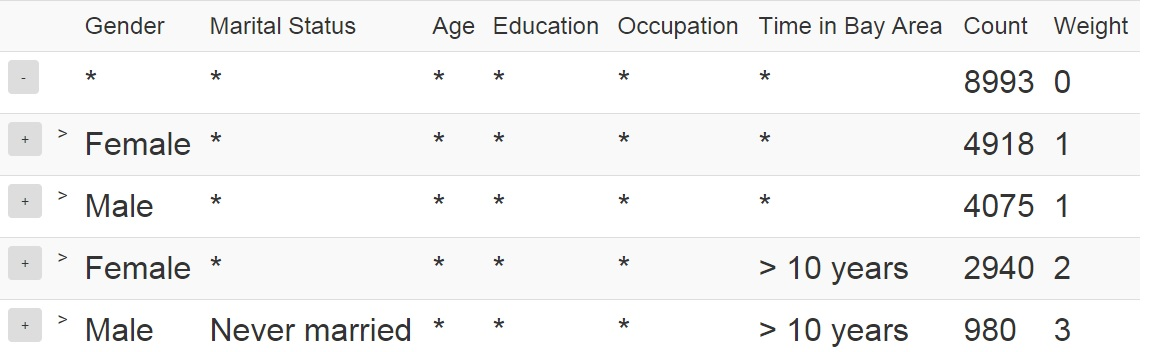
\includegraphics[width=80mm,frame]{graphs/screenshots6col/empty_expansion.jpg}
\caption{Summary after clicking on the empty rule \label{fig:uiexample1}}
\vspace{-10pt}
\end{figure} 

\begin{figure}
\centering
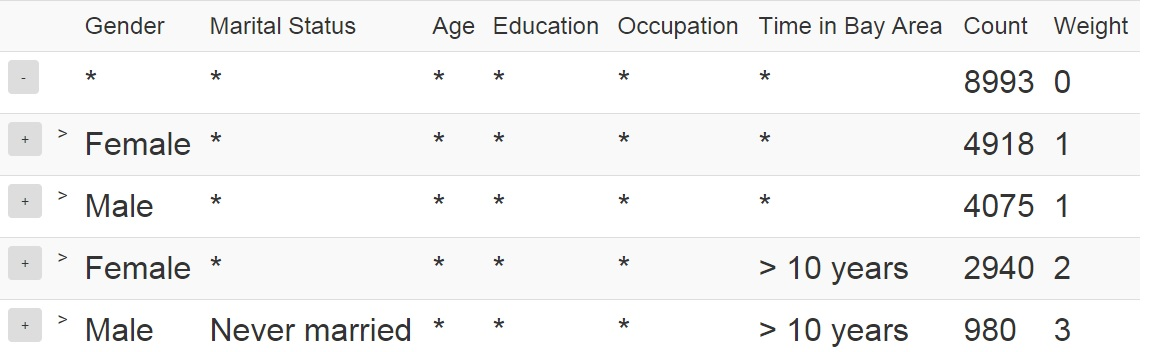
\includegraphics[width=80mm,frame]{graphs/screenshots6col/empty_expansion.jpg}
\caption{Star expansion on `Education' Column \label{fig:uiexamplestar}}
\vspace{-10pt}
\end{figure}

Now suppose the user decides to further explore the table, by looking at education related information of females in the dataset. Say the user clicks on the $\star$ in the `Education' column of the second rule. This opens up Figure~\ref{fig:uiexamplestar} that shows the number of females with different levels of education, for the $4$ most frequent levels of education among females. Instead of expanding the `Education' column, if the user had simply expanded the third rule, it would have displayed Figure~\ref{fig:uiexamplerule}. 

\subsubsection{Weighting functions}
Our system can display optimal rule lists for any monotonic weighting function. By default, we assign a rule weight equal to its size. In this section, we consider other weighting functions. 

We first try the weighting function given by:
$$W(r) = \sum_{c \in C : r(c) \neq \star} \lceil \text{log}_2(|c|) \rceil$$ where $|c|$ refers to the number of distinct possible values in column $c$. This function gives higher weight to rules that have non-$\star$ values in columns that have many possible values. The rule summary for this weighting is in Figure~\ref{fig:weigtingbitwise} (contrast with Figure~\ref{fig:uiexample1}). The weighting scheme gives low weight for non-$\star$ values in binary columns, like the gender column. Thus, this summary instead gives us information about the Marital Status/Time in Bay Area/Occupation columns instead of the Gender column like in Figure~\ref{fig:uiexample1}.  

The other weighting function we try is given by:
$$W(r) = \text{Min}(0, \text{Size}(r) - 1)$$
This gives us Figure~\ref{fig:weightingsizeminusone}. This weighting gives a $0$ weight to rules with a single non-$\star$ value, and thus forces the algorithm to finds good rules having at least $2$ non-$\star$ values. As a result, we can see that our system only displays rules having $2$ or $3$ non-$\star$ values, unlike Figure~\ref{fig:uiexample1} which has two rules displaying the total number of males and females, that have size $1$.

A regular drill down can be thought of as a special case of smart drill-down with the right weighting function and number of rules\papertext{ (see technical report for details)}\techreporttext{. Specifically, if we want to perform a regular drill down on a column $C$ that has $n$ distinct values, then we set the number of rules to be displayed ($k$) to $n$. The weighting function $W$ is set such that $W(r) = 1$ if rule $r$ has $C$ instantiated, and $0$ otherwise. This ensures that all displayed rules have $C$ instantiated (with no other column $C'$ instantiated unless there is a functional dependency from $C$ to $C'$), and that each displayed rule has a distinct value of $C$. This effectively gives us a regular drill-down on $C$}. We use this to perform a drill down on the `Age' column using our experimental prototype. The result is shown in Figure~\ref{fig:drilldownexample}. We can contrast it with Figure~\ref{fig:uiexample1}; the latter gives information about multiple columns at once and only displays high count values. Regular drill down on the other hand, serves a complementary purpose by focusing on detailed evaluation of a single column.

%TODO: Give application examples for different weighting functions
%TODO: Say somewhere, that we haev drop-down list of common weighting functions in the user interface, with column selects and unselects.


\begin{figure}
%\vspace{-10pt}
\centering
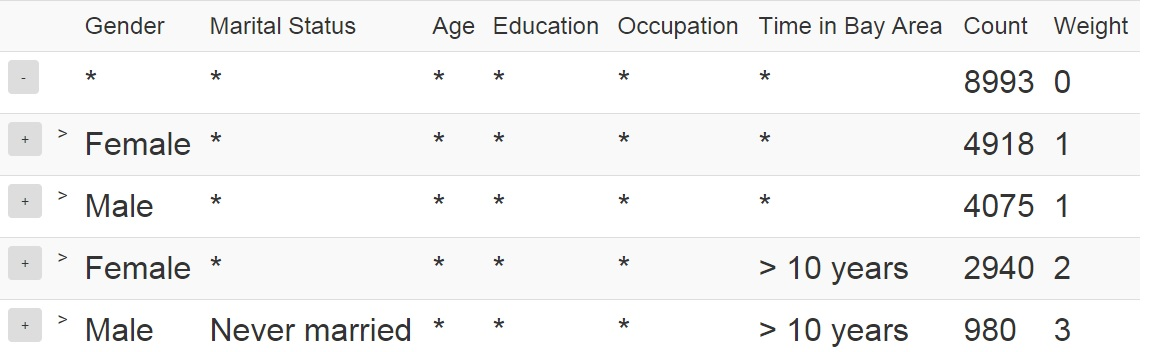
\includegraphics[width=80mm,frame]{graphs/screenshots6col/empty_expansion.jpg}
\caption{A rule expansion \label{fig:uiexamplerule}}
\vspace{-10pt}
\end{figure}

\begin{figure}
\centering
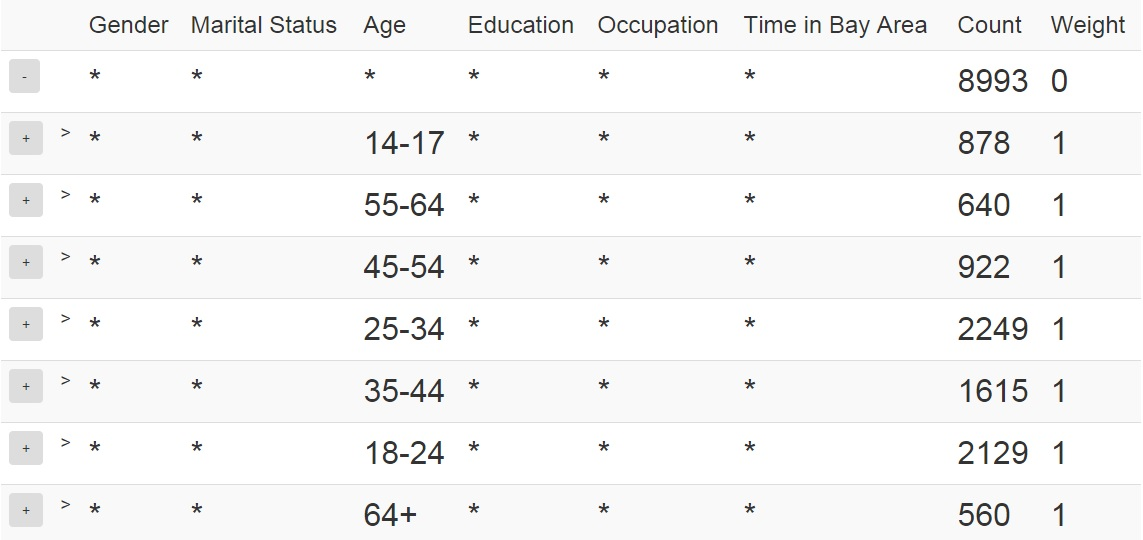
\includegraphics[width=80mm,frame]{graphs/screenshots6col/age_drilldown.jpg}
\caption{A regular drill down on Age\label{fig:drilldownexample}}
\vspace{-10pt}
\end{figure}



% TODO: Add the experiment where you compare to vanilla a priori.
\subsection{Quantitative Study}\label{sec:quantitative_study}
The performance of our algorithm depends on various parameters, such as $m_w$ (the max weight) and $minSS$ (minimum required sample size). We now study the effects of these parameters on the computation time and accuracy of our algorithm. We use the Marketing and Census datasets. The Marketing dataset is relatively small with around $9000$ tuples, whereas the Census dataset is quite large, with $2.5$ million tuples. The accuracy of our algorithm depends on $m_w$ and $minSS$, rather than the underlying database size. The worst case running time for large datasets is close to the time taken for making one pass on the dataset. When we expand a rule using an existing sample in memory, the running time is small and only depends on $minSS$ rather than on the dataset size.

\subsubsection{Effects of $m_w$}
Our algorithm for finding the best marginal rule takes an input parameter called $m_w$. The algorithm is guaranteed to find the best marginal rule as long as its weight is $\leq m_w$, but runs faster for smaller values of $m_w$. We now study the effect of varying $m_w$ on the speed of our algorithm running on a Dell XPS L702X laptop with 6GB RAM and an Intel i5 2.30GHz processor.

We fix a weighting function $W$, and a value of $m_w$. For that value of the $W$ and $m_w$ parameters, we find the time taken for expanding the empty rule. We repeat this procedure $10$ times and take the average value of the running times across the $10$ iterations. This time is plotted against $m_w$, for $W(r) = \text{Size}(r)$ and $W(r) = \sum_{c \in C : r(c) \neq \star} \lceil \text{log}_2(|c|) \rceil$ in Figure~\ref{fig:mw_speed}. The figure shows that running time seems to be approximately linear in $m_w$. 

For the Census dataset, the running time is dominated by time spent in making a pass through the $2.5$ million tuples to create the first sample. The response time for the next user click should be quite small, as the sample created for the first expansion can usually be re-used for the next rule expansion.

The value of $m_w$ required to ensure a correct answer is equal to the maximum weight of a selected rule. Thus, for size scoring on the Marketing dataset, according to Figure~\ref{fig:uiexample1}, we require $m_w \geq 3$. For the second weighting function, according to Figure~\ref{fig:weigtingbitwise}, the minimum required value of $m_w$ is $10$. At these values of $m_w$, we see that the expansion takes $1.5$ seconds and about $0.25$ seconds respectively. Of course, the minimum value of $m_w$ we can use is not known to us beforehand. But even if we use more conservative values of $m_w$, say $6$ and $20$ respectively, the running times are about $1.5$ and $0.5$ seconds respectively.

\begin{figure}
\centering
  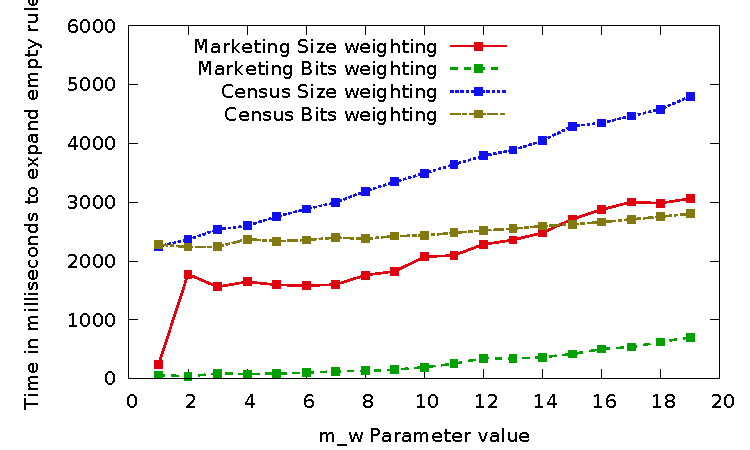
\includegraphics[scale=0.46]{graphs/mw_speed.pdf}%change height to 2 inch for actual paper, 5 inch for single column
  \caption{Running time for different values of parameter $m_w$ \label{fig:mw_speed}}
\vspace{-10pt}
\end{figure}

\subsubsection{Effects of $minSS$}
We now study the effects of the sampling parameter $minSS$. This parameter tells the SampleHandler the minimum sample size on which we run BRS. Higher values of $minSS$ cause our system to use bigger samples, which increases the accuracy of count estimates for displayed rules, but also correspondingly increases computation time. 

We consider one value of $minSS$ and one weight function $W$ at a time. For those values of $minSS$ and $W$, we drill down on the empty rule and measure the time taken. We also measure the percent error in the estimated counts of the displayed rules. That is, for each displayed rule $r$, if the displayed (estimated) count if $c_1$ and the actual count (computed separately on the entire table) is $c_2$, then the percent error for rule $r$ is $\frac{100 \times |c_1-c_2|}{c_2}$. We consider the average of percent errors over all displayed rules. For each value of $minSS$ and $W$, we drill down on the empty rule and find the computation time and percent error $50$ times, and take the average value for time and error over those $50$ iterations. This average time is plotted against $minSS$, for $W(r) = \text{Size}(r)$ and $W(r) = \sum_{c \in C : r(c) \neq \star} \lceil \text{log}_2(|c|) \rceil$ in Figure~\ref{fig:minSS_speed}(a). The average percent error is plotted against $minSS$, for $W(r) = \text{Size}(r)$ and $W(r) = \sum_{c \in C : r(c) \neq \star} \lceil \text{log}_2(|c|) \rceil$ in Figure~\ref{fig:minSS_error_percent}(b). 

\begin{figure}
\centering
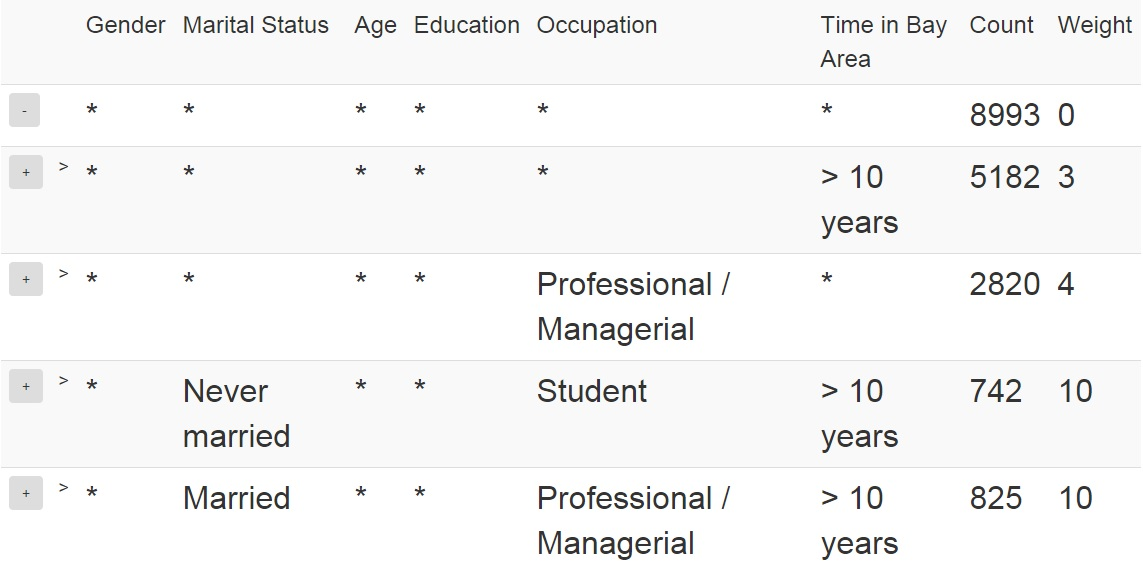
\includegraphics[width=80mm,frame]{graphs/screenshots6col/bits_scoring.jpg}
\caption{Bits scoring\label{fig:weigtingbitwise}}
\vspace{-15pt}
\end{figure}

\begin{figure}
\vspace{-10pt}
\centering
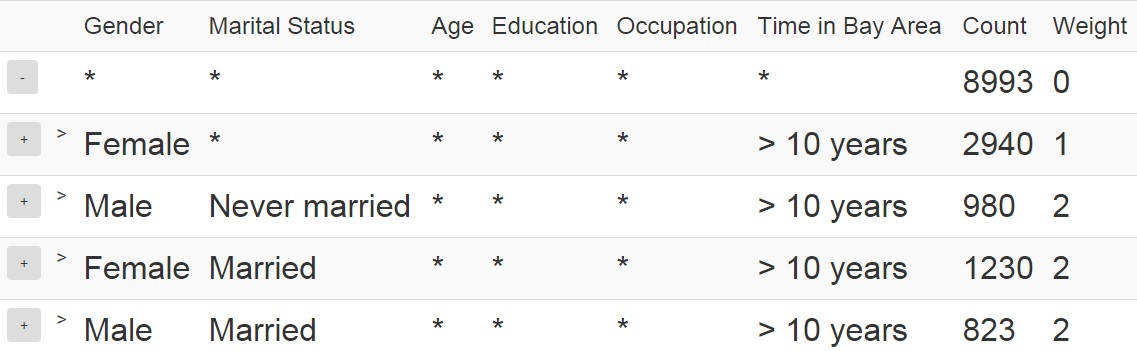
\includegraphics[width=80mm,frame]{graphs/screenshots6col/min2_scoring.jpg}
\caption{Size minus one weighting \label{fig:weightingsizeminusone}}
\vspace{-10pt}
\end{figure}

Figure~\ref{fig:minSS_speed}(a) shows that sampling gives us noticeable time savings. The percent error decreases approximately as $\frac{1}{\sqrt{minSS}}$, which is again expected because the standard deviation of estimated $Count$ is approximately inversely proportional to the square root of sample size.

In addition, we measure the number of incorrect rules per iteration. If the correct set of rules to display is $r_1, r_2, r_3$ and the displayed set is $r_1, r_3, r_4$ then that means there is one incorrect rule. We find the number of incorrect displayed rules across $50$ iterations, and display the average value in Figure~\ref{fig:minSS_error_rule}(c). This number for the Marketing dataset is almost always $0$ for the Size weighting function, and between $1$ and $2$ for the Bits weighting function. For the Census dataset, it is around $1$ for $minSS \leq 1000$ and falls to about $0.3$ for larger values of $minSS$. Note that even when we display an `incorrect' rule, it is usually the $5^{th}$ or $6^{th}$ best rule instead of one of the top $4$ rules, which still results in a reasonably good summary of the table.

\begin{figure*}[!ht]
\centering
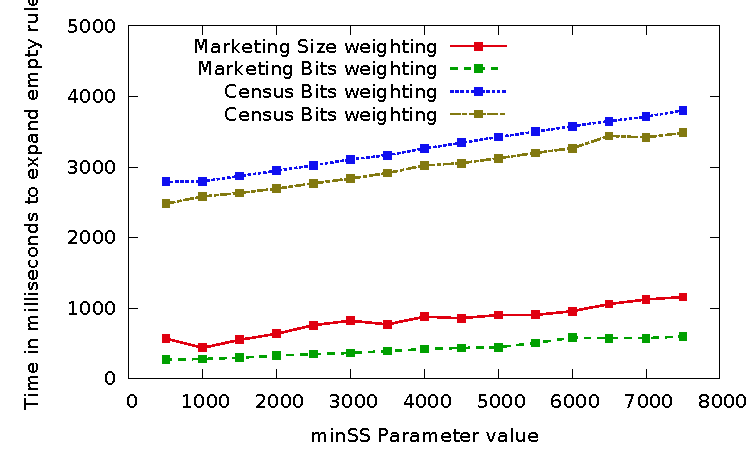
\includegraphics[scale=0.46]{graphs/minSS_speed.pdf}
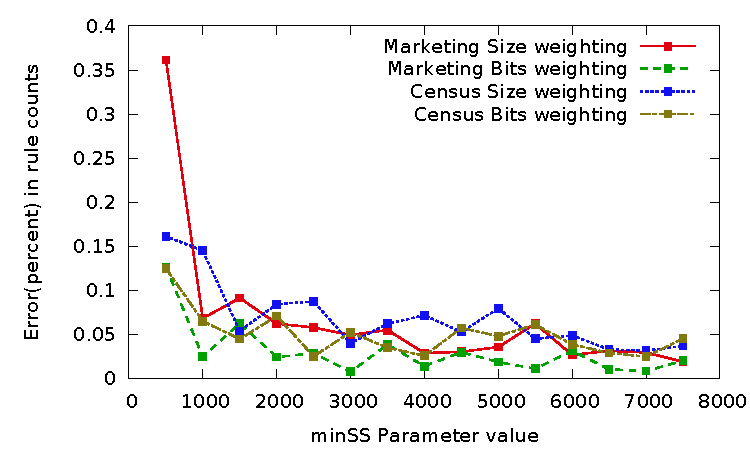
\includegraphics[scale=0.46]{graphs/minSS_error_percent.pdf}
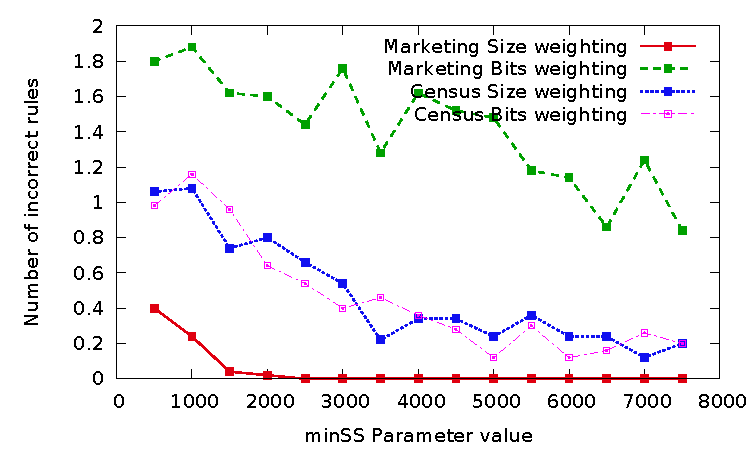
\includegraphics[scale=0.46]{graphs/minSS_error_rule.pdf}
\caption{(a) Running time for different values of parameter $minSS$ (b) Error in Count for different values of parameter $minSS$ (c) Average number of incorrect rules for different values of parameter $minSS$ \label{fig:minSS_speed}\label{fig:minSS_error_percent} \label{fig:minSS_error_rule}}
\vspace{-10pt}
\end{figure*}

\subsubsection{Scaling properties of our algorithms}
The computation time for a smart drill-down is linear in both the table size $|T|$ and in parameter $minSS$. That is, the runtime can be written as $a \times |T| + b \times minSS$ where $a$ and $b$ are constants. In the worst-case where we cannot form a sample from main memory and need to re-create a sample, $a$ stands for the time taken to read data from hard disk. That is, $a \times |T|$ is the time taken to make a single sequential scan over the table on disk. The constant $b$ is bigger than $a$, because BRS makes multiple passes over the sample, while creating a sample only requires a single pass over the table.

When the $|T|$ is small, the runtme is dominated by the $b \times minSS$ term, as seen for the Marketing Dataset in Figure~\ref{fig:minSS_speed}(a). When $|T|$ is large relative to $minSS$, like for the Census Dataset, the runtime is dominated by the $a \times |T|$ term (this is when we need to create a fresh sample from hard disk). When we have a few million tuples, our total runtime is only a few seconds. But if the dataset consisted of billions of tuples, the process of reading the table to create a sample could itself take a very long time. To counteract this, we could preprocess the dataset by down-sampling it to only a million tuples, and perform the summarization on the million tuple sample (which also effectively summarizes the billion tuple table).

\techreporttext{
\section{Extensions}\label{sec:extensions}
\subsection{Dealing with Numerical Attributes}\label{sec:extensions-numerical}
Our algorithm assumes that all attributes are categorical in nature. Attributes that have a large domain tend to have a smaller tuple count per value, and hence don't appear in rule summaries. Thus our algorithm does not summarise information about numerical attributes. 

However, we can modify the algorithm to deal with numerical attributes. Suppose we have a numerical attribute $A$. A simple approach is to create buckets for values of $A$. We choose a number of buckets $b$, and divide the range of values of $A$ into $b$ intervals, each corresponding to a bucket. We can create buckets having an equal range size, or decide their range such that there is an approximately equal number of tuples in each bucket. Then we can use our algorithm, treating the bucket number as a categorical attribute. This is already done in our MD dataset, where numerical attributes like age are divided into buckets ($18-24$, $25-34$ and so on).

\subsection{Using Sum instead of Count}\label{sec:extensions-sum}
Throughout the paper, we define the total score of a rule-list using the marginal counts of rules in the list, and display the count of each rule in our table summary. However, if we have a numerical column (i.e. a `measure' column) in the table, it is straightforward to extend our summary to the `Sum' aggregate over that column instead. Suppose we are given a measure column $c_m$. Then the {\em Sum} for a rule can be defined to be the sum of $c_m$ values over all tuples covered by the rule. {\em MSum} of a rule $r$ in a rule-list $R$ is the sum of $c_m$ values over all tuples covered by $r$ and not covered by any rule in $R$ that occurs before $r$. The Score for $R$ becomes $\text{Score}(R) = \sum_{r\in R} MSum(r,R)W(r)$. Algorithm~\ref{algo:best-rule-set} can be modified to find the best rule set using the new definition of Score, simply by replacing $Count(r)$ by $Sum(r)$ and computing sum and marginal sum instead of count and marginal count in each pass over the table.
}

\section{Related Work}\label{sec:related}

There has been work on finding cubes to browse in OLAP systems~\cite{Sarawagi:2001:UMA:767141.767148, Sarawagi00user-adaptiveexploration, Sarawagi98discovery-drivenexploration}. This work, along with other existing work~\cite{Mampaey:2011:TMI:2020408.2020499} focuses on finding values that occur more often or less often that expected from a max-entropy distribution. The work does not guarantee good coverage of the table, since it rates infrequently occurring sets of values as highly as frequently occurring ones. Some other data exploration work~\cite{sellam:meet} focuses on finding attribute values that divide the database in equal sized parts, while we focus on values that occur as frequently as possible. 

There is work on constructing `explanation tables', sets of rules that co-occur with a given binary attribute of the table~\cite{DBLP:journals/pvldb/GebalyAGKS14}. This work again focuses on displaying rules that will cause the resulting max entropy distribution to best approximate the actual distribution of values. A few vision papers~\cite{data-deluge, cetintemel2013query} suggest frameworks for building interactive data exploration systems. Some of these ideas, like maintaining user profiles, could be integrated into smart drill down. Reference~\cite{DBLP:conf/edbt/CandanCQS09} proposes an extension to OLAP drill-down that takes visualization real estate into account, by clustering attribute values. But it focuses on expanding a single column at a time, and relies on a given value hierarchy for clustering.

Some related work~\cite{DBLP:journals/debu/GolabKS11, Golab:2008:GNT:1453856.1453900} focuses on finding minimum sized Tableaux that provide improved support and confidence for conditional functional dependencies. There has also been work~\cite{Bu:2005:MSH:1083592.1083644, Lakshmanan:2002:GMA:1287369.1287435, DBLP:conf:kdd:XiangJFD08, Geerts04tilingdatabases} on finding hyper-rectangle based covers for tables. In both these cases, the emphasis is on completely covering or 
summarizing the table, suffering from the same problems as traditional drill down in that the user may be presented with
too many results. The techniques in the former case may end up picking rare ``patterns'' if they have high confidence, and in the latter case do not scale well to a large number of attributes (in their case, $\geq 4$). 

Several existing papers also deal with the problem of frequent itemset mining~\cite{apriori, 1411744, Han:2000:MFP:342009.335372}. Vanilla frequent itemset mining is not directly applicable to our problem because the flexible user-specified objective function emphasizes coverage of the table rather than simply frequent itemsets.  However, we do leverage ideas from the a-priori algorithm~\cite{apriori} as applicable. Several extensions have been proposed to the a-priori algorithm, including those for dealing with numerical attributes~\cite{Srikant:1996:MQA:233269.233311, Miller:1997:ARO:253260.253361}. We can potentially use these ideas to improve handing of numerical attributes in our work. Unlike our paper, there has been no work on dynamically maintaining samples for interaction in the frequent itemset literature, since frequent itemset mining is a one-shot problem.

There has also been plenty of work on pattern mining. Several papers~\cite{Vreeken:2011:KMI:1969593.1969615,Bringmann:2007:ICDM,Yan:2005:SIP:1081870.1081907} propose non-interactive schemes that attempt to find a one shot summary of the table. These schemes usually consume a large amount of time processing the whole table, rather than allowing the user to slowly steer into portions of interest. In contrast, our work is interactive, and includes a smart memory manager that can use limited memory effectively while preparing for future requests.

Our Smart Drill-Down operator is tunable because of the flexible weighting function, but the monotonicity of the weighting function and the use of $MCount$, still make it possible for us to get an approximate optimality guarantee for the rules we display. In contrast, much of the existing pattern mining work~\cite{Goethals:2011:MFI:2020408.2020529,Tatti:2014:FRI:2676651.2656261,DeBie:2010:FMI:1816112.1816117} is not not tunable enough, providing only a fixed set of interestingess parameters. On the other hand, reference~\cite{Leeuwen:2012:DSS:2347179.2347243} allows a fully general scoring function, necessitating the use of heuristics with no optimality guarantees, and very time consuming algorithms. 
A lot of pattern mining work~\cite{Goethals:2011:MFI:2020408.2020529,Yan:2005:SIP:1081870.1081907,Vreeken:2011:KMI:1969593.1969615} also focuses on itemsets rather than Relational Data, which does not allow the user to express interest in certain `columns' over others.

We use sampling to find approximate estimates of rule counts. Various other database systems~\cite{Acharya:1999:AAQ:304182.304581, Agarwal:2013:BQB:2465351.2465355} use samples to find approximate results to SQL aggregation queries. These systems create samples in advance and only update them when the database changes. In contrast, we keep updating our samples on the fly, as the user interacts with our system. There is work on using weighted sampling~\cite{6691587} to create samples favouring data that is of interest to a user, based on the user's history. In contrast, we create samples at run time in response to the user's commands.

\section{Conclusion}\label{sec:conclusion}
We have presented a new data exploration operator called smart drill down.
Like traditional drill down, it allows an analyst
to quickly discover interesting value patterns (rules) that occur frequently
(or that represent high values of some metric attribute)
across diverse parts of a table.

We presented an algorithm for optimally selecting rules
to display, as well as a scheme for performing such selections
based on data samples. Working with samples makes smart drill down
relatively insensitive to the size of the table.

Our experimental results on our experimental prototype show that smart drill down
is fast enough to be interactive under various
realistic scenarios. We also showed that the accuracy is high
when sampling is used, and when the maximum weight ($m_w$)
approximation is used. Moreover, we have a tunable parameter $minSS$ that the user can tweak to tradeoff performance of smart drill down for the accuracy of the rules.

				
\bibliographystyle{abbrv}
\bibliography{smartDrillDown}


\vspace{17pt}

\begin{comment}
\begin{wrapfigure}{l}{0.15\textwidth}
%   \begin{center}

\includegraphics[height=3.5cm, width=2.7cm]{./figures/hector.pdf}
%   \end{center}
\end{wrapfigure}

Hector Garcia-Molina is the Leonard Bosack and Sandra Lerner Professor in the Departments of Computer Science and Electrical Engineering at Stanford University, Stanford, California. He was the chairman of the Computer Science Department from January 2001 to December 2004. From 1997 to 2001 he was a member the President's Information Technology Advisory Committee (PITAC). From August 1994 to December 1997 he was the Director of the Computer Systems Laboratory at Stanford. From 1979 to 1991 he was on the faculty of the Computer Science Department at Princeton University, Princeton, New Jersey. His research interests include distributed computing systems, digital libraries and database systems. He received a BS in electrical engineering from the Instituto Tecnologico de Monterrey, Mexico, in 1974. From Stanford University, Stanford, California, he received in 1975 a MS in electrical engineering and a PhD in computer science in 1979. He holds an honorary PhD from ETH Zurich (2007). Garcia-Molina is a Fellow of the Association for Computing Machinery and of the American Academy of Arts and Sciences; is a member of the National Academy of Engineering; received the 1999 ACM SIGMOD Innovations Award; is a Venture Advisor for Onset Ventures, is a member of the Board of Directors of Oracle, and is a member of the State Farm Technical Advisory Council.
\medskip


\begin{wrapfigure}{l}{0.15\textwidth}
%   \begin{center}
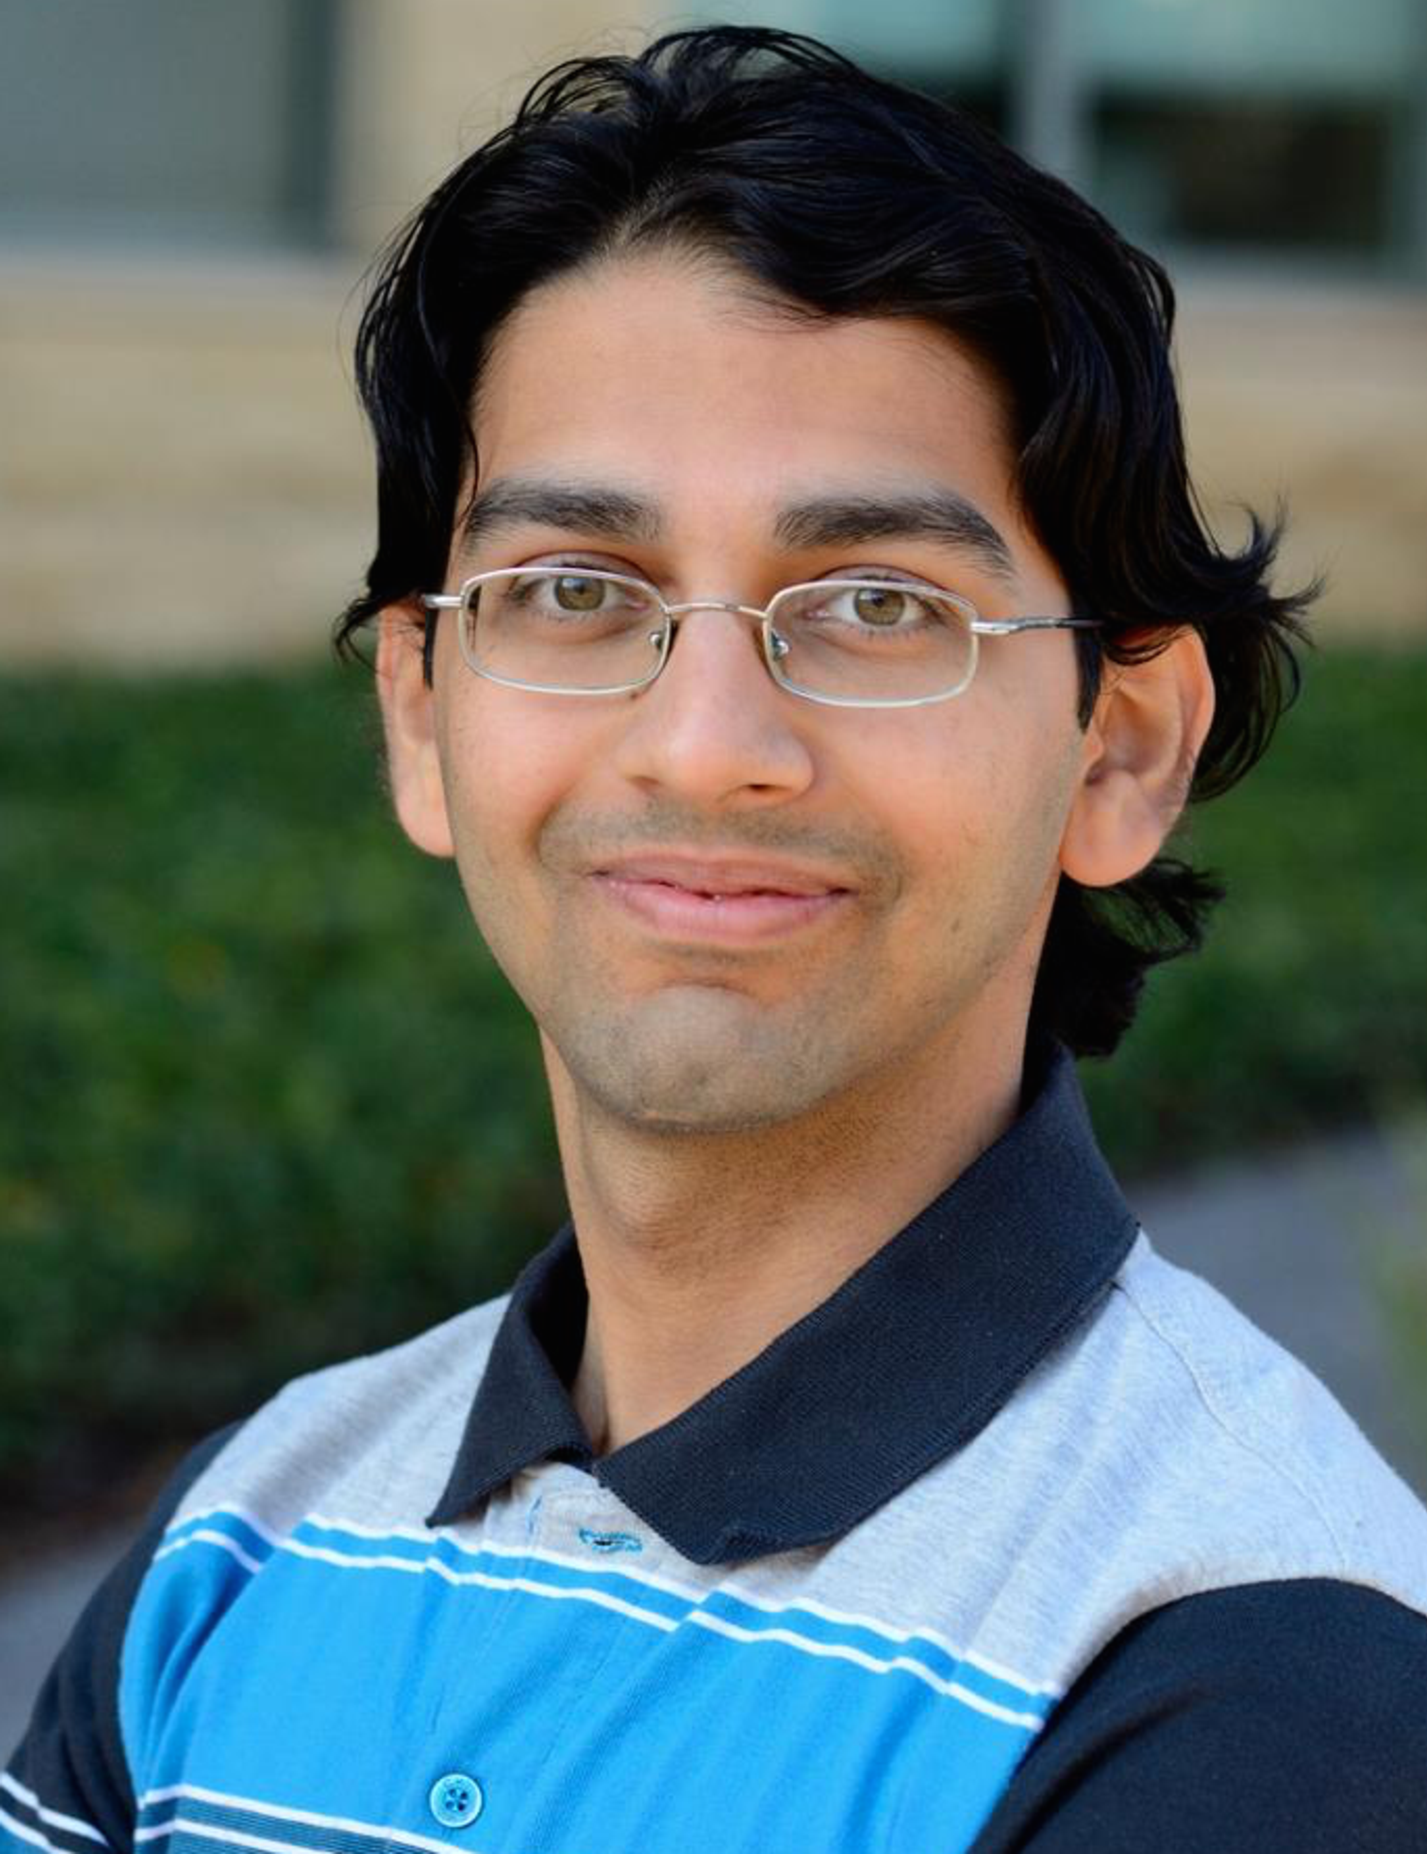
\includegraphics[height=3.5cm, width=2.7cm]{./figures/Manas.pdf}
%   \end{center}
\end{wrapfigure}

Manas Joglekar is a fifth year PhD student in the Computer Science Department at Stanford University. Manas' advisor is Prof. Hector Garcia-Molina, and his research interests include Crowdsourcing, Data Quality Evaluation and Database Theory. Prior to that, he received a B. Tech in Computer Science and Engineering from the Indian Institute of Technology Bombay, in 2011.
\medskip


\begin{wrapfigure}{l}{0.15\textwidth}
%   \begin{center}
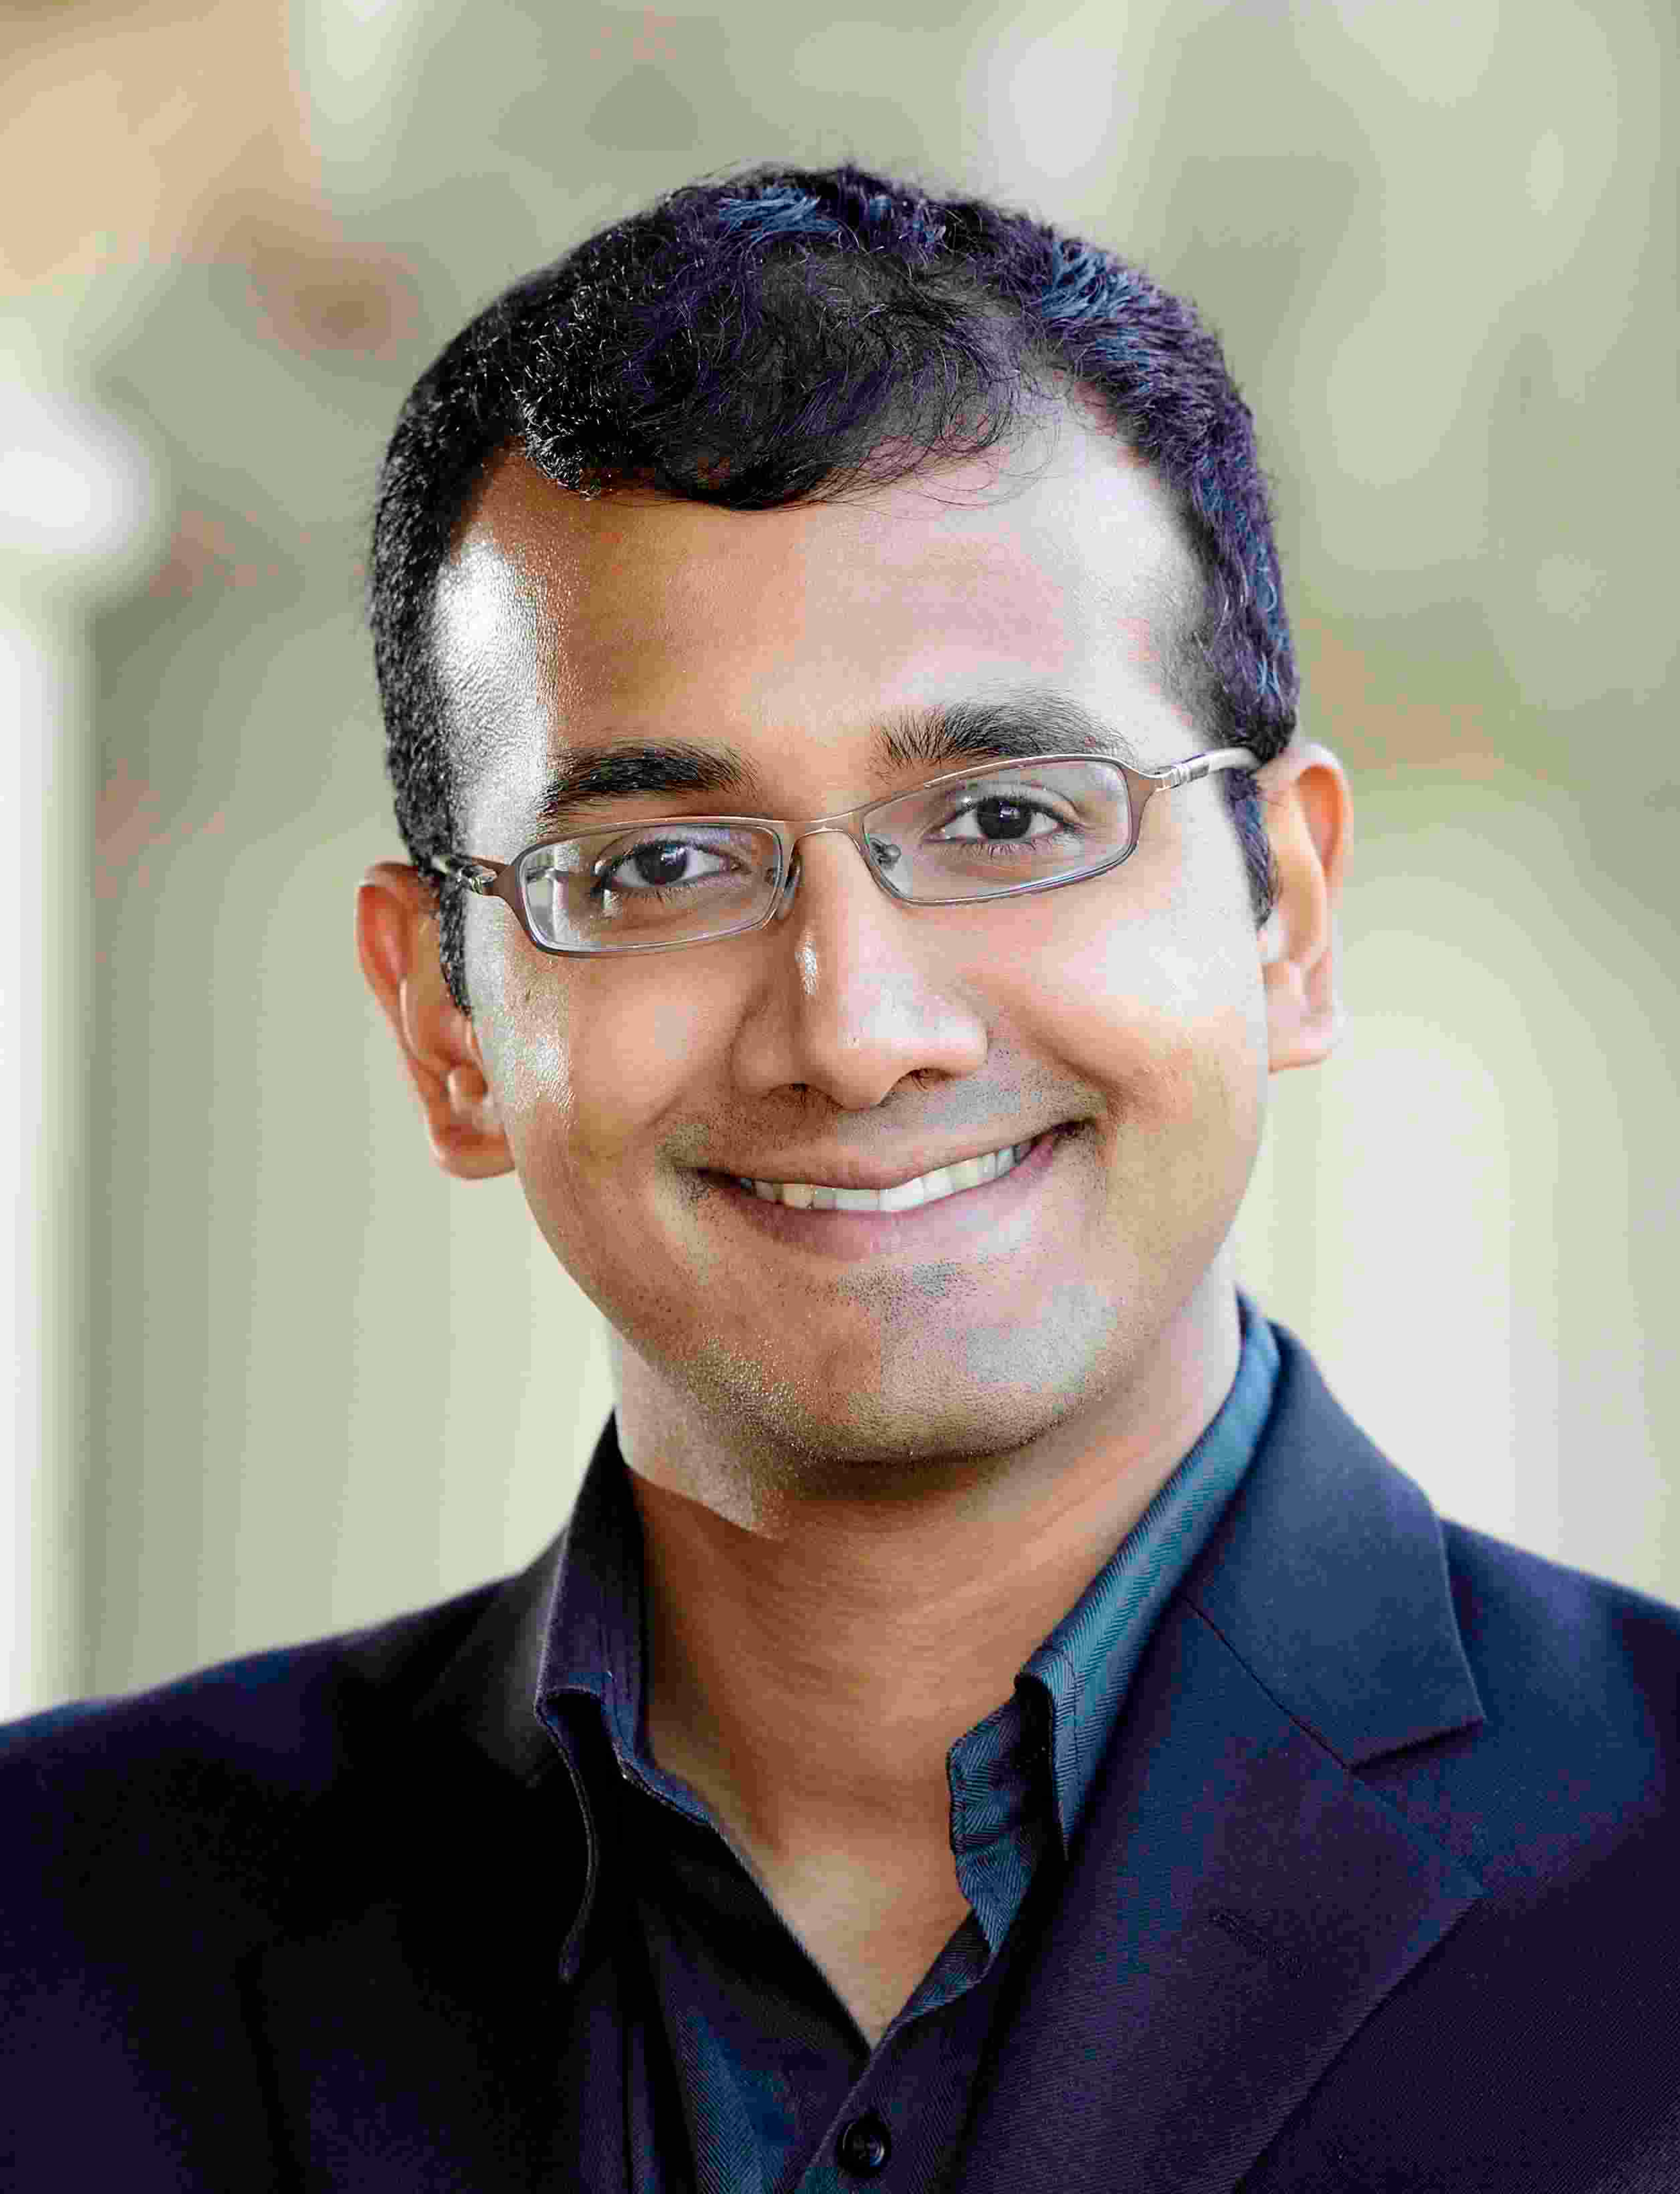
\includegraphics[height=3.5cm, width=2.7cm]{./figures/aditya.pdf}
%   \end{center}
\end{wrapfigure}

Aditya Parameswaran is an Assistant Professor in Computer Science at the University of Illinois (UIUC). He spent the 2013-14 year visiting MIT CSAIL and Microsoft Research New England, after completing his Ph.D. from Stanford University, advised by Prof. Hector Garcia-Molina. He is broadly interested in data analytics, with research results in human computation, visual analytics, information extraction and integration, and recommender systems. 
Aditya is a recipient of the Arthur Samuel award for the best dissertation in CS at Stanford (2014), the SIGMOD Jim Gray dissertation award (2014), the SIGKDD dissertation award runner up (2014), a Google Faculty Research Award (2015), the Key Scientific Challenges Award from Yahoo! Research (2010), three best-of-conference citations (VLDB 2010, KDD 2012 and ICDE 2014), the Terry Groswith graduate fellowship at Stanford (2007), and the Gold Medal in Computer Science at IIT Bombay (2007). His research group is supported with funding from by the NIH, the NSF, and Google.
\medskip
\end{comment}


\end{document}
			
		













